\documentclass[12pt,spanish,Letterpaper,openany]{book}
\usepackage{lmodern}
\usepackage{setspace}
\setstretch{0.85}
\usepackage{amssymb,amsmath}
\usepackage{ifxetex,ifluatex}
\usepackage{fixltx2e} % provides \textsubscript
\ifnum 0\ifxetex 1\fi\ifluatex 1\fi=0 % if pdftex
  \usepackage[T1]{fontenc}
  \usepackage[utf8]{inputenc}
\else % if luatex or xelatex
  \ifxetex
    \usepackage{mathspec}
  \else
    \usepackage{fontspec}
  \fi
  \defaultfontfeatures{Ligatures=TeX,Scale=MatchLowercase}
    \setmainfont[Scale=1.0]{Corbel}
    \setsansfont[]{Corbel}
    \setmonofont[Mapping=tex-ansi]{Corbel}
\fi

\makeatletter
\renewcommand\mainmatter{\clearpage\@mainmattertrue\pagenumbering{arabic}}
\renewcommand\frontmatter{\clearpage\@mainmatterfalse\pagenumbering{arabic}}
\renewcommand\backmatter{\clearpage\@mainmatterfalse}
\makeatother

%\usepackage{etoolbox}
%\makeatletter
%\patchcmd{\@smemmain}{\cleardoublepage}{\clearpage}{}{}
%\patchcmd{\@smemmain}{\cleardoublepage}{\clearpage}{}{}
%\patchcmd{\@smemfront}{\cleardoublepage}{\clearpage}{}{}
%\patchcmd{\@smemfront}{\cleardoublepage}{\clearpage}{}{}
%\makeatother

\setlength{\parindent}{0em}

\usepackage{graphicx}
\usepackage{booktabs}
\usepackage{multicol}
\usepackage{doc}
\usepackage{float}
\usepackage{tcolorbox} 
\usepackage{lipsum}
\usepackage{tikz}
\usepackage{nonfloat}

\usepackage{pdfpages}

\usepackage[
contents={},
opacity=1,
scale=1.5,
color=blue!90
]{background}
\usepackage{lipsum}
\usepackage{ifthen}

\usepackage{xcolor}
\usepackage[pagestyles]{titlesec}

\renewpagestyle{plain}[\normalsize\sffamily\bfseries\slshape]{
  \setfoot{}{\color{black}{\thepage}}{}}

\newpagestyle{myps}[\normalsize\sffamily\bfseries\slshape]{
  \setfoot{}{\color{black}{\thepage}}{}}
  
\pagestyle{myps}


\usepackage{framed}
\definecolor{colorlinetitle}{HTML}{a87e00}%{a87e00}%
\definecolor{textlinetitle}{HTML}{061769}%{061769}%{061769}%
\definecolor{fondo}{HTML}{041d57}%
\definecolor{newfondo}{HTML}{3d0718}%
\colorlet{shadecolor}{fondo!81!}


% use upquote if available, for straight quotes in verbatim environments
\IfFileExists{upquote.sty}{\usepackage{upquote}}{}
% use microtype if available
\IfFileExists{microtype.sty}{%
\usepackage{microtype}
\UseMicrotypeSet[protrusion]{basicmath} % disable protrusion for tt fonts
}{}
\usepackage[inner=12.7mm,outer=12.7mm,top=23mm,bottom=18.5mm]{geometry}
\usepackage{hyperref}
\hypersetup{unicode=true,
            pdftitle={Revista digital de la escuela de ingeniería en Ciencias y Sistemas},
            pdfauthor={Escuela Ingenieria en Ciencias y Sistemas},
            pdfborder={0 0 0},
            breaklinks=true}
\urlstyle{same}  % don't use monospace font for urls
\ifnum 0\ifxetex 1\fi\ifluatex 1\fi=0 % if pdftex
  \usepackage[shorthands=off,main=spanish]{babel}
\else
  \usepackage{polyglossia}
    % Fallback por si no viene definido desde Pandoc
  \setmainlanguage{spanish}
\fi
\usepackage{natbib}
\bibliographystyle{plainnat}
\usepackage{longtable,booktabs}
\IfFileExists{parskip.sty}{%
\usepackage{parskip}
}{% else
\setlength{\parindent}{0pt}
\setlength{\parskip}{6pt plus 2pt minus 1pt}
}
\setlength{\emergencystretch}{3em}  % prevent overfull lines
\providecommand{\tightlist}{%
  \setlength{\itemsep}{0pt}\setlength{\parskip}{0pt}}
\setcounter{secnumdepth}{5}
% Redefines (sub)paragraphs to behave more like sections
\ifx\paragraph\undefined\else
\let\oldparagraph\paragraph
\renewcommand{\paragraph}[1]{\oldparagraph{#1}\mbox{}}
\fi
\ifx\subparagraph\undefined\else
\let\oldsubparagraph\subparagraph
\renewcommand{\subparagraph}[1]{\oldsubparagraph{#1}\mbox{}}
\fi

%%% Use protect on footnotes to avoid problems with footnotes in titles
\let\rmarkdownfootnote\footnote%
\def\footnote{\protect\rmarkdownfootnote}


  \title{Ingeniería social: el lado humano de las filtraciones de datos.}
    \author{Jorge Mario Castañeda Cragua y Kevin Martin Samayoa Urizar}
      \date{2025-10-27}

% no title page
\AtBeginDocument{\let\maketitle\relax}


% === Secciones automáticas ===
\usepackage{pdfpages}    % ya lo usas
\usepackage{ifthen}      % ya lo usas
\usepackage{background}  % ya lo usas

% Macro: \SectionPDF{<path/pdf>}{<pagina_limite>}
% Muestra el PDF de la sección e impone el fondo hasta "pagina_limite-1"
\newcommand{\SectionPDF}[2]{%
  % Incrusta el PDF completo de la sección
  \includepdf[pages=-]{#1}%
  % Aplica fondo en cada página hasta el límite indicado
  \AddEverypageHook{%
    \ifthenelse{\value{page}<#2}{%
      \ifthenelse{\isodd{\value{page}}}{%
        \backgroundsetup{scale=1, color=white, opacity=1, angle=0, contents={%
          
\includegraphics[width=\paperwidth,height=\paperheight]{latex/background_numberimpar.pdf}}}%
      }{%
        \backgroundsetup{scale=1, color=white, opacity=1, angle=0, contents={%
          
\includegraphics[width=\paperwidth,height=\paperheight]{latex/background_numberpar.pdf}}}%
      }%
    }{}%
    \BgMaterial
  }%
}


\usepackage{caption2}
\captionsetup{%
labelsep=colon,%
font={footnotesize},%
aboveskip=0.4\baselineskip,%
belowskip=0\baselineskip,% deve essere 0 perché regolo lo spazio dal testo con \intextsep
}%

\usepackage{booktabs}
\usepackage{longtable}

\usepackage{indentfirst}
\setlength{\parindent}{1em}
\usepackage{enumitem}
\setlist[itemize]{labelindent = \parindent, leftmargin=*}

%\usepackage{framed,color}
%\definecolor{shadecolor}{RGB}{248,248,248}

\renewcommand{\textfraction}{0.05}
\renewcommand{\topfraction}{0.8}
\renewcommand{\bottomfraction}{0.8}
\renewcommand{\floatpagefraction}{0.75}

\renewcommand{\chaptername}{Artículo}
\addto\captionsspanish{\renewcommand{\chaptername}{Artículo}}
\addto\captionsspanish{\renewcommand{\contentsname}{Índice General}}


\frenchspacing
\tolerance=5000
\multicoltolerance=3000 

\raggedbottom
\raggedcolumns

\setlength{\columnsep}{1em}
%We want a rule between columns.
%\setlength\columnseprule{.4pt}

%Tambien queremos asegurarnos de que un nuevo entorno multicols 
%encuentre suficiente espacio en la parte inferior de la pagina.
\setlength\premulticols{6\baselineskip}

%Al equilibrar columnas, ignoramos las soluciones que son 
%demasiado malas. Ademas, si la ultima columna es demasiado mala, 
%la tipeamos sin estirar.
\setcounter{columnbadness}{7000}
\setcounter{finalcolumnbadness}{7000}

\newcommand{\prefacetitlecommand}%
{\titleformat{\chapter}[display]%
{\bfseries\large\color{colorlinetitle}}%
{\relax}%
{0ex}%
{{\titlerule[1.2pt]}\filright\color{textlinetitle}}[\color{colorlinetitle}\vspace{0.5ex}{\titlerule[1.2pt]}]%
}


\newcommand{\articletitlecommand}%
{\titleformat{\chapter}[display]%
{\bfseries\tiny\raggedright\color{white}}%
{\relax}%
{0ex}%
{}[\color{white}\vspace{0ex}{\titlerule[0pt]}]%
}



\newcommand{\sectionCenter}%
{\titleformat{\section}[block]%
{\bfseries\large\color{textlinetitle}\filcenter}%
{\relax}%
{0ex}%
{\empty}%
}


\newcommand{\sectionRight}%
{\titleformat{\section}[block]%
{\bfseries\large\color{textlinetitle}}%
{\relax}%
{0ex}%
{\empty}%
}


\newcommand{\subsectionRight}%
{\titleformat{\subsection}[block]%
{\bfseries\normalsize\color{textlinetitle}}%
{\relax}%
{0ex}%
{\empty}%
}


\usepackage{titletoc}
\titlecontents{chapter}[3em]
{\vspace{5mm}}
{\normalsize\contentslabel[\color{textlinetitle}\thecontentslabel]{2em}\color{black}\itshape\normalsize}
{\color{black}\itshape\normalsize}
{\color{colorlinetitle}\titlerule*[.3pc]{.}\color{black}\contentspage}

\newcommand{\tcolorboxcommand}{\begin{tcolorbox}[sharp corners=uphill, colback=newfondo, colframe=newfondo, arc=6mm, boxrule=0mm, boxsep=0mm]}

\newcommand{\photocommand}[2]{%
\fcolorbox[HTML]{DCEEA7}{DCEEA7}{%
\begin{minipage}{95.19mm}%
	\hspace{1mm}%
	\begin{minipage}{22.49mm}%
		\vspace{1mm}%
		\includegraphics[width=22.49mm, height=31.96mm]{#1}%
		\vspace{1mm}%
	\end{minipage}%
	\hspace{2.4mm}%
	\begin{minipage}{68.80mm}%
		#2
	\end{minipage}%
	\hspace{0.5mm}%
\end{minipage}%
}%
}

\definecolor{fondobiography}{HTML}{DCEEA7}

\NewDocumentEnvironment{photobiography}{m O{}}%
{%
\begin{tcolorbox}[colback=fondobiography, colframe=fondobiography, width=97.19mm, boxsep=-2mm, arc=0mm]
\begin{minipage}{95.19mm}%
	%\hspace{1mm}%
	\begin{minipage}{22.49mm}%
		\vspace{2mm}%
		\includegraphics[width=22.49mm, height=31.96mm]{#1}%
		\vspace{2mm}%
	\end{minipage}%
	\hspace{2.4mm}%
	\begin{minipage}{68.80mm}%
	#2%
}%
{%
	\end{minipage}%
	%\hspace{0.5mm}%
\end{minipage}%
\end{tcolorbox}
}


\newcommand{\spacetext}{\vspace{8.1mm}}
\newcommand{\minimalspacetext}{\vspace{1mm}}
\newcommand{\spaceelevenmilis}{\vspace{11mm}}
\newcommand{\spacetenmilis}{\vspace{10mm}}
\newcommand{\spaceninemilis}{\vspace{9mm}}
\newcommand{\spaceeightmilis}{\vspace{8mm}}
\newcommand{\spacesevenmilis}{\vspace{7mm}}
\newcommand{\spacesixmilis}{\vspace{6mm}}
\newcommand{\spacefivemilis}{\vspace{5mm}}
\newcommand{\spacefourmilis}{\vspace{4mm}}
\newcommand{\spacethreemilis}{\vspace{3mm}}
\newcommand{\spacetwomilis}{\vspace{2mm}}
\newcommand{\spaceinitialeditorialcontenido}{\vspace{8.1mm}}
\newcommand{\spaceoneminus}{\vspace{-1mm}}
\newcommand{\spacetwominus}{\vspace{-2mm}}
\newcommand{\spacefourminus}{\vspace{-4mm}}
\newcommand{\hideFromPandoc}[1]{#1}
\hideFromPandoc{ \let\Begin\begin \let\End\end }
\newcommand{\minipagepartone}{\begin{minipage}[c]{3cm}}
\newcommand{\minipagetwocolumn}{\noindent\begin{minipage}[c]{\columnwidth}}
\newcommand{\minipageparttwo}{\end{minipage}\begin{minipage}[c]{12cm}}
\newcommand{\minipageparttwochapter}{\end{minipage}\begin{minipage}[c]{15cm}}
\newcommand{\minipageendpart}{\end{minipage}}
\newcommand{\firstparteditorial}{\begin{longtable}[]{@{}ll@{}}\endhead\begin{minipage}[t]{0.47\columnwidth}\raggedright}
\newcommand{\firstparttwoeditorial}{\begin{longtable}[l]{@{}ll@{}}\endhead\begin{minipage}[t]{0.47\columnwidth}\raggedright}
\newcommand{\midleparteditorial}{\end{minipage} & \begin{minipage}[t]{0.47\columnwidth}\raggedright}
\newcommand{\lastparteditorial}{\end{minipage}\end{longtable}}

\newcommand{\HRule}{\begin{center}\rule{0.5\linewidth}{0.2mm}\end{center}}

\begin{document}
\maketitle

% \pagestyle{plain}

\includepdf{images/cover.pdf}

\AddEverypageHook{%
\ifthenelse{\value{page}<5}%
{\ifthenelse{\isodd{\value{page}}}%
  	{\backgroundsetup{scale=1, color=white, opacity=1, angle=0, contents={
\includegraphics[width=\paperwidth,height=\paperheight]{latex/background_numberimpar.pdf}}}}%
  	{\backgroundsetup{scale=1, color=white, opacity=1, angle=0, contents={
\includegraphics[width=\paperwidth,height=\paperheight]{latex/background_numberpar.pdf}}}}%
}{}%
\BgMaterial}

\hypersetup{
  unicode=true,
  pdftitle={Revista digital de la escuela de ingeniería en Ciencias y Sistemas},
  pdfauthor={Escuela Ingenieria en Ciencias y Sistemas},
  pdfborder={0 0 0},
  breaklinks=true,
  linkcolor=black, % TOC y refs
  urlcolor=gray    % solo URLs
}

%%%%%%{
%%%%%%\setcounter{tocdepth}{0}
%%%\tableofcontents
%%%}
%%%%%%%%%
\prefacetitlecommand

\titlespacing*{\chapter} {0pt}{0pt}{2pt}

\titleformat{\chapter}[display]
{\normalfont\color{black} \bfseries}
{\empty}
{0pt}
{\filcenter\Huge}

\spacetenmilis
\spacetenmilis
\spacetenmilis
\spacetenmilis

\begin{center}
\includegraphics[width=1\linewidth]{images/organigrama} \end{center}

\chapter*{Editorial}\label{editorial}
\addcontentsline{toc}{chapter}{Editorial}

\begin{center}
\includegraphics[width=1\linewidth]{images/editorial_html} \end{center}

\setcounter{tocdepth}{0}
\tableofcontents

\articletitlecommand

\titlespacing*{\chapter}{0pt}{-60pt}{4pt}

\SectionPDF{images/seccion1.pdf}{15}

\chapter{Docencia aumentada: IA, personalización y ética en el aula}\label{entrevista01_JaimeChamale}

\begin{center}
\includegraphics[width=1\linewidth]{autores_seleccionados/e1} \end{center}

\begin {multicols}{2}

\textbf{\emph{YouTube:}} \url{https://youtu.be/0Rj48TXLdiQ}

\section{Entrevista}\label{entrevista}

\textbf{¿Quién es Jaime Ismael Chamale?}

Soy Jaime Ismael Chamale Morales, ingeniero en sistemas, con una maestría en Seguridad de la Información. Actualmente soy catedrático en la Universidad Panamericana y cuento con más de siete años de experiencia en el desarrollo de soluciones para distintas áreas del mercado laboral, como banca, seguros y sector público.

Desde hace varios años imparto clases en la Universidad Panamericana, donde aplico conocimientos como análisis de datos, automatización de tareas y desarrollo de software. En mis cursos integro la inteligencia artificial como asistente de planificación y apoyo creativo.

La IA me permite analizar los contenidos curriculares de los cursos para evaluar su vigencia y proponer mejoras. Con base en ese análisis estructuro planificaciones didácticas, establezco objetivos y competencias, y defino el esquema completo del curso. Además, la IA me ayuda a alinear metodologías de enseñanza y a crear borradores de recursos (diapositivas, guías, lecturas, preguntas y ejercicios). Todo esto ahorra tiempo en tareas repetitivas y me permite dedicar más energía al acompañamiento personalizado de los estudiantes.

\textbf{¿Cómo definiría la inteligencia artificial y qué importancia tiene hoy en la educación?}

Defino la inteligencia artificial como una disciplina que busca desarrollar sistemas capaces de realizar tareas usualmente realizadas por humanos, como el aprendizaje continuo, el razonamiento y la resolución de problemas. En educación, su importancia es valiosa y transformadora: no es solo una herramienta, sino un catalizador de cambio de paradigma.

La IA permite automatizar tareas administrativas y repetitivas, liberando tiempo valioso para los docentes. Ofrece retroalimentación inmediata sobre las actividades, y adapta el contenido al ritmo, estilo e intereses de cada estudiante. También facilita la tutoría personalizada y el análisis de tendencias en el desempeño, lo que ayuda a detectar patrones y realizar intervenciones oportunas cuando surgen dificultades.

\textbf{¿Qué lo motivó a interesarse en el uso de IA para la enseñanza?}

Principalmente, la búsqueda de soluciones a dos problemas centrales: la masificación de las aulas y la dificultad para atender necesidades individuales en grupos numerosos. A esto se suma la brecha de acceso a la tecnología, que afecta la formación. La IA ofrece herramientas para abordar ambos desafíos y fomenta competencias, pensamiento crítico y creatividad, superando enfoques centrados solo en la memorización.

\textbf{¿Cómo ha cambiado la forma de crear y compartir contenido educativo con la IA?}

El cambio ha sido radical gracias a la democratización de la creación de materiales. Antes, producir recursos diversos era complejo y demandaba mucho tiempo. Hoy, un docente puede generar en minutos textos, cuestionarios, imágenes o planes didácticos, con solo indicar a la IA lo que desea. Asimismo, compartir y distribuir esos recursos es más sencillo, y las plataformas sugieren alternativas útiles para el aula.

La creación de contenidos pasó de ser estática y manual a un proceso rápido y dinámico. La IA permite esbozar borradores y planes de acción que luego ajustamos a las necesidades del curso. Además, facilita diferenciar lecciones según los niveles de aprendizaje, definir competencias específicas y promover pensamiento crítico y creatividad.

\textbf{¿Cómo ha cambiado la forma de crear y compartir contenido educativo con la IA?}

He utilizado la IA para generar ejercicios, cuestionarios y juegos interactivos, creando múltiples versiones de un mismo recurso para distintos grupos. También la empleo para disminuir el plagio, reescribir o readecuar contenidos, idear lluvias de ideas, diseñar mapas de ruta y elaborar ejemplos, casos de uso o relatos que inspiran el debate.

En lo visual, la uso para crear imágenes y elementos gráficos como diagramas, infografías y organigramas. La IA permite explicitar objetivos por recurso y alinearlos con el plan didáctico o la malla curricular, favoreciendo una secuencia temática coherente. Esto impulsa un enfoque por proyectos, mientras que la teoría puede prepararse con apoyo de la IA.

\textbf{¿Qué ventajas ofrece frente a los métodos tradicionales?}

Las principales ventajas son la velocidad y la eficiencia. Ahora podemos crear contenido con rapidez, apoyándonos en la IA para consultar fuentes y generar versiones alternativas. También mejora la diversificación de recursos para diferentes estilos de aprendizaje (auditivo, visual o kinestésico) y facilita crear juegos interactivos o asistentes que guían la resolución de problemas.

Otra ventaja es el aprendizaje adaptativo: el proceso deja de ser genérico y se ajusta a las necesidades de cada estudiante. Para el docente, los cuestionarios automatizados aceleran la calificación y permiten brindar retroalimentación inmediata, algo que antes requería más tiempo y dificultaba responder a cada alumno de forma oportuna.

\textbf{¿Cómo ha cambiado el rol del docente al integrar la IA?}

El docente ha pasado de ser la única voz en el aula a desempeñar roles de facilitador, mentor y tutor. Con la IA disponemos de múltiples perspectivas y vías para abordar un tema y llegar a los mismos resultados. El docente ahora es también creador, evaluador y curador de contenidos, responsable de filtrar lo que comparte en clase.

Además, debe facilitar la interacción entre estudiantes y desarrollar habilidades blandas. Otro rol emergente es el de intérprete de datos: analizar la información que brindan las herramientas de IA para monitorear el progreso y tomar decisiones pedagógicas.

\textbf{¿Cómo puede la IA ayudar a personalizar los materiales según el ritmo de aprendizaje?}

La IA permite personalizar en tiempo real a partir del desempeño de los estudiantes. Con ello identificamos necesidades, patrones y conceptos no comprendidos. Podemos definir mapas de ruta que orientan los prerrequisitos antes de avanzar a temas complejos; si el estudiante se desorienta, cuenta con una guía para retomar el camino.

Asimismo, ajustamos los ejercicios al nivel de exigencia adecuado y generamos adaptaciones de accesibilidad (por ejemplo, para dificultades visuales o auditivas). Todo esto facilita el proceso de enseñanza y lo hace más inclusivo.

\textbf{¿Cuáles son los principales riesgos o limitaciones del uso de IA en educación?}

Entre los riesgos están los sesgos, que pueden perpetuarse o amplificarse en los modelos y dar lugar a contenidos inadecuados. También la deshumanización si hay uso excesivo, lo cual puede erosionar el proceso educativo. Existe el riesgo de brecha digital entre quienes tienen acceso a estas herramientas y quienes no, generando desigualdad. Finalmente, preocupa la dependencia excesiva y la pérdida de habilidades sociales.

\textbf{¿Cómo asegurar la calidad y evitar desinformación o plagio?}

Es clave formar y capacitar a docentes y estudiantes en alfabetización digital para verificar y validar la información, revisar fuentes y cuestionar resultados. El docente debe actuar como filtro y supervisor del contenido generado por los estudiantes, comprobando que provenga de fuentes confiables.

Podemos usar herramientas de verificación para detectar plagio y, a la vez, fomentar la autoría, incentivando la creación de contenidos propios.

\textbf{¿Qué papel juega la ética en la creación de contenido con IA?}

La ética es un pilar fundamental en todo el proceso. Debemos ser transparentes sobre cuándo y cómo usamos la IA, y proteger la privacidad: evitar introducir datos personales o confidenciales en plataformas públicas. La ética implica responsabilidad en el uso, así como verificar la calidad e idoneidad del contenido generado.

\textbf{¿Cómo imagina la educación en los próximos 5 a 10 años con IA?}

Imagino un sistema híbrido con tutores omnipresentes (incluso en realidad virtual) que asistan de forma continua, tanto en el aula como desde el hogar. Las clases estarían centradas en proyectos, mientras la IA prepararía la teoría y la retroalimentación sería constante e inmediata. Este enfoque haría al sistema más competente, a la vez que potencia la humanización y el desarrollo de habilidades sociales.

\textbf{¿Qué competencias deberían desarrollar estudiantes y docentes para aprovechar la IA?}

Estudiantes:

\begin{itemize}
\tightlist
\item
  Pensamiento crítico y escepticismo saludable para cuestionar y verificar fuentes.
\item
  Gestión de la información para formular preguntas adecuadas y analizar/sintetizar respuestas.
\item
  Creatividad e innovación para no depender en exceso de la IA.
\end{itemize}

Docentes:

\begin{itemize}
\tightlist
\item
  Alfabetización digital para comprender las herramientas y aprovecharlas al máximo con mirada crítica.
\item
  Mentoría y guía socioemocional para potenciar habilidades del estudiante.
\item
  Diseño de experiencias de aprendizaje apoyadas en datos y en la interpretación de la analítica educativa.
\end{itemize}

\textbf{Mensaje final de Jaime Chamale}

Invito a los docentes a mantenerse en capacitación constante para hacer buen uso de las herramientas de IA, y a fomentar el espíritu crítico y analítico en los estudiantes. La IA debe ser un complemento para mejorar el aprendizaje, no una dependencia.

\end {multicols}

\medskip

\HRule

\medskip

\chapter{Más allá de los libros: la inteligencia artificial como el nuevo compañero en el aprendizaje}\label{pareja41}

\begin{center}
\includegraphics[width=1\linewidth]{autores_seleccionados/a1} \end{center}

\begin {multicols}{2}

\textbf{\emph{Palabras clave:}} Educación adaptativa, personalización, sesgo algorítmico, automatización.

\section{Introducción}\label{introducciuxf3n}

La inteligencia artificial se ha convertido en un aspecto importante dentro de varios campos de la sociedad moderna, que va desde el entretenimiento hasta la vida académica de las personas, y si bien existen temas éticos en relación a su uso en cada uno de estos entornos, es innegable la necesidad de aprender a utilizarlo y aprovecharlo como una herramienta más de nuestro día a día.

La educación y el aprendizaje es uno de los campos más afectados por esta nueva tecnología y si bien presenta grandes beneficios, es necesario contextualizar su implementación de una manera adecuada, de tal manera que se facilite el acceso a soluciones tanto a estudiantes como docentes sin impactar de manera negativa en su pensamiento crítico y cognitivo.

\section{Artículo}\label{artuxedculo}

\bigskip

\textbf{La penetración de la inteligencia artificial en la educación}

La inteligencia artificial (IA) ha estado presente en la educación en donde se ha ido
integrando profundamente en el aprendizaje y la enseñanza en todo el mundo. Esta herramienta mejora la experiencia de aprendizaje, aumenta la eficiencia académica, automatiza tareas administrativas y hace que la educación sea más accesible.{[}1{]}

Recientemente estadísticas publicadas por Statista : el portal de estadísticas en línea demostró que un 86\% de los estudiantes ya utilizan herramientas de IA en su aprendizaje. Las cifras por sí solas demuestran que el 24\% utilizan IA a diario, el 54\% la utiliza a diario o semanalmente y por último el 54\% la utiliza al menos semanalmente.{[}2{]}

\begin {flushleft}
\noindent\begin{minipage}[c]{\columnwidth}

\begin{center}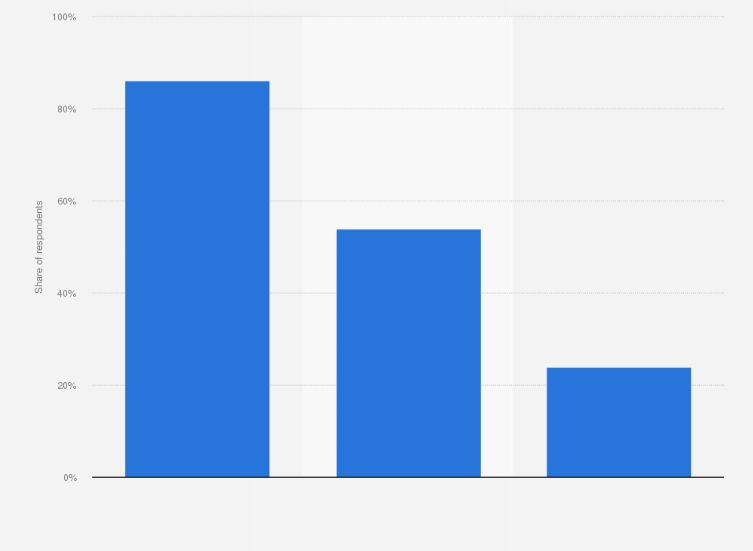
\includegraphics[width=1\linewidth]{imagenes_articulos_seleccionados/A1/p1} \end{center}
\figcaption{Porcentaje de estudiantes que usan IA para la escuela a nivel global.}

\end{minipage}
\end {flushleft}

\bigskip

\textbf{La inteligencia artificial como una herramienta para la personalización}

Al hacer uso de la inteligencia artificial se busca proporcionar diseños de clases
personalizadas, dinámicas y enfocadas en una participación estudiantil más activa. El docente actúa como un arquitecto de experiencias, mientras que la tecnología le aporta ideas esteactúa como un soporte para realizar un acercamiento de contenidos a distintos estilos de
aprendizaje.{[}3{]}

El objetivo es no perder la vinculación humana, la IA nos ofrece una gran información valiosa sobre el rendimiento o el nivel de actividad de cada estudiante, pero ese lazo afectivo lo construye el docente quien pregunta, se acerca y fomenta esa confianza con los estudiantes.

\bigskip

\textbf{Las responsabilidades éticas de los docentes y estudiantes}

Las aplicaciones de IA deben ser monitoreadas de una manera muy crítica, de forma que se eviten sesgos o usos indebidos de los datos. El docente aumentado enseña a mirar la tecnología con precaución y a reflexionar sobre sus implicaciones sociales, no solo únicamente se trabaja la asignatura de turno, también la información de un alumnado que sepa cuestionarse sobre los avances tecnológicos con responsabilidad. Esto implica reconocer desafíos como la equidad, la privacidad y los sesgos, abordándolos con prácticas como auditorías de datos, transparencia y acompañamiento docente.

\begin {flushleft}
\noindent\begin{minipage}[c]{\columnwidth}

\begin{center}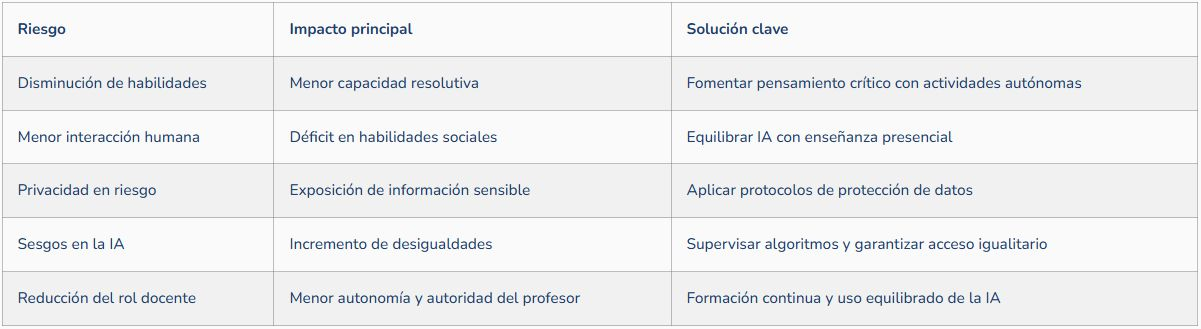
\includegraphics[width=1\linewidth]{imagenes_articulos_seleccionados/A1/p2} \end{center}
\figcaption{Riesgos del uso excesivo de la IA.}

\end{minipage}
\end {flushleft}

El estudio, titulado ``Uso de IA generativa y resultados de exámenes'', encontró que los estudiantes que utilizaron herramientas de este tipo llegaron a obtener un promedio de 6.71 puntos menos (de 100 posibles) que aquellos que no lo realizaron. Esto nos sugiere que las herramientas IA pueden interferir en el crecimiento de aprendizaje y afectar negativamente los resultados de los exámenes.{[}1{]}

\bigskip
\bigskip

\section{Conclusiones}\label{conclusiones}

La inteligencia artificial está moldeando el futuro de la educación al ofrecernos herramientas poderosas que mejoran el aprendizaje, simplifican las tareas y apoyan tanto a los educadores como a los estudiantes. La IA es un valioso asistente en la educación, en el trabajo, en los negocios, impulsando innovaciones y preservando esa esencia humana que hace que el aprendizaje sea verdaderamente empírico y significativo. Sin embargo, es necesario abordar cuestiones como la integridad académica, la seguridad y la igualdad, y la clave del éxito reside en una integración responsable.

\section{Referencias}\label{referencias}

\begin{itemize}
\item
  {[}1{]} Cherneha, Sofia. ``AI in Education : Transforming Learning and Teaching in 2025'' ScrumLaunch Blog, Febrero,2025. Accedido el 28 de marzo de 2025. \href{https://www.scrumlaunch.com/blog/ai-in-education-transforming-learning-and-teaching-in-2025}{https://scrumlaunch.com}.
\item
  {[}2{]} Korhonen, Veera. ``Share of Students Using IA for Schoolwork Worldwide as of July 2024'' Statista, Junio,2025. Accedido el 23 de junio de 2025. \href{https://www.statista.com/statistics/1498309/usage-of-ai-by-students-worldwide/}{https://www.statista.com}
\item
  {[}3{]} Equipo Observatorio ProFuturo.``El docente aumentado: la alianza entre docentes e inteligencia artificial''. Observatorio Profuturo, Abril,2025. Accedido el 9 de abril de 2025. \href{https://profuturo.education/observatorio/tendencias/el-docente-aumentado-la-alianza-entre-docentes-e-inteligencia-artificial/}{https://www.profuturo.education.com}
\end{itemize}

\end {multicols}

\medskip

\chapter{La revolución silenciosa: Asistentes virtuales transformando el panorama educativo}\label{pareja22}

\begin{center}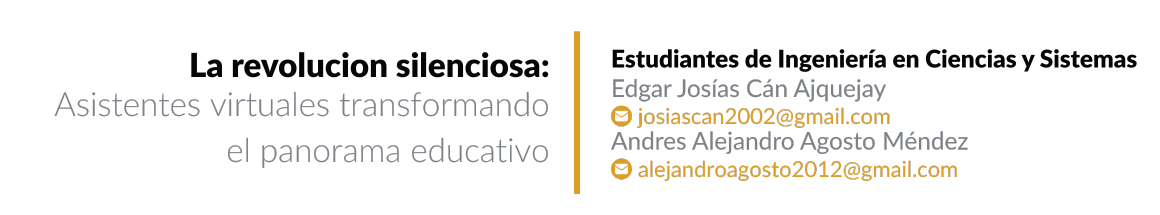
\includegraphics[width=1\linewidth]{autores_seleccionados/a2} \end{center}

\begin {multicols}{2}

\textbf{\emph{Palabras clave:}} Asistentes Virtuales Educativos, Educación, Evaluación Automática, Privacidad de Datos, Inteligencia Artificial.

\section{Introducción}\label{introducciuxf3n-1}

La evolución de la inteligencia artificial (IA), impulsada por el auge de ChatGPT en 2022, ha transformado múltiples ámbitos, incluida la educación. Los asistentes virtuales se han vuelto aliados cotidianos en escuelas y universidades, ofreciendo apoyo personalizado a estudiantes y docentes. Facilitan nuevas formas de aprendizaje, así como guías de estudio y estrategias que potencian la enseñanza.

No obstante, surge la pregunta: ¿son aliados que enriquecen la educación o un posible reemplazo del docente? Ante el avance acelerado de la tecnología educativa, urge evaluar con rigor su integración. El análisis debe ponderar oportunidades (acceso, personalización, eficiencia) y desafíos (ética, sesgos, privacidad). Este trabajo aborda ese balance en el contexto académico actual.

\section{Artículo}\label{artuxedculo-1}

\bigskip

\textbf{Adopción y estadísticas actuales}

Según la Figura 3.1, más del 56\% de los estudiantes, tanto en Estados Unidos como en el resto del mundo, utilizan herramientas de inteligencia artificial (IA) como ChatGPT para sus estudios. Aunque un 40.6\% todavía no las usa por dudas sobre su precisión, la IA se está volviendo más sofisticada y confiable.

\begin {flushleft}
\noindent\begin{minipage}[c]{\columnwidth}

\begin{center}
\includegraphics[width=1\linewidth]{imagenes_articulos_seleccionados/A2/p1} \end{center}
\figcaption{Porcentaje de estudiantes universitarios que han usado IA en tareas o exámenes.}

\end{minipage}
\end {flushleft}

Esto sugiere que adaptarse a este nuevo método de aprendizaje merece la pena, ya que la integración de asistentes virtuales personalizados en las escuelas podría desmentir la creencia de que la IA no es una herramienta de aprendizaje efectiva y precisa. Además, con la implementación de estos modelos en las universidades y escuelas a través de asistentes virtuales adaptados a su modelo de aprendizaje académico. Puede rebatir la opinión de que la IA no es adecuada para el autoaprendizaje.

\bigskip

\textbf{Arquitectura y tecnología de los asistentes virtuales}

Los asistentes virtuales educativos integran procesamiento de lenguaje natural, aprendizaje automático y bases de conocimiento estructuradas. Su efectividad depende de algoritmos de inferencia y de bases de datos que utilizan ontologías formales para ofrecer razonamiento automático. Esta arquitectura requiere servidores de alto rendimiento y una infraestructura robusta que permita el análisis en tiempo real.

\bigskip

\textbf{Implementaciones institucionales}

Diversas instituciones han adoptado estas tecnologías. La Universidad de Michigan utiliza asistentes virtuales para aprendizaje autodirigido y soporte académico. Carnegie Mellon ha desarrollado sistemas tutoriales inteligentes capaces de adaptar contenidos según el progreso del estudiante. El Instituto de Tecnología de Georgia emplea chatbots para responder preguntas frecuentes y orientar procesos administrativos. Además, la Universidad de Stanford y Harvard han explorado asistentes en cursos en línea, mientras que la UNESCO promueve su uso en proyectos globales de educación digital.

\bigskip

\textbf{Funcionalidades y capacidades avanzadas}

Los asistentes virtuales ofrecen funciones como revisión de exámenes, tutorías personalizadas y calificación automatizada. También utilizan algoritmos de recomendación basados en el rendimiento histórico del estudiante. En la Universidad Estatal de Arizona, chatbots especializados proporcionan retroalimentación inmediata en cursos de matemáticas y ciencias. El MIT, por su parte, ha integrado asistentes en laboratorios virtuales, permitiendo experimentos guiados y simulaciones interactivas.

\bigskip

\textbf{Desafíos y perspectivas futuras}

Aunque los beneficios son amplios, persisten desafíos como sesgos algorítmicos, privacidad de datos y la necesidad de supervisión constante. El 59.8\% de los estudiantes de ingeniería utiliza IA generativa en proyectos de diseño, lo que muestra un rápido crecimiento. El futuro apunta hacia la convergencia con realidad aumentada, análisis de emociones y algoritmos basados en neurociencia cognitiva. Estas innovaciones demandarán infraestructuras distribuidas y marcos éticos sólidos.

\bigskip
\bigskip

\section{Conclusiones}\label{conclusiones-1}

Los asistentes virtuales educativos no reemplazan, sino que complementan la enseñanza al ofrecer soporte personalizado y ampliar las capacidades pedagógicas. A pesar de limitaciones técnicas como los sesgos algorítmicos, su impacto crecerá bajo la estricta supervisión humana. El éxito de integración requiere un enfoque equilibrado que conserve la interacción humana, la cual es esencial en la educación. Para lograrlo, las instituciones deben establecer marcos éticos claros y la formación docente en competencias digitales se vuelve crucial. El futuro de la educación dependerá de la sinergia entre la innovación tecnológica y la experiencia pedagógica. La colaboración entre desarrolladores, educadores y estudiantes es fundamental para crear soluciones beneficiosas. En última instancia, el éxito de estas tecnologías se medirá por su capacidad de democratizar el acceso a una educación de calidad y personalizada.

\section{Referencias}\label{referencias-1}

\begin{itemize}
\item
  {[}1{]} Essel, Harry Barton, Dimitrios Vlachopoulos, y Akosua Tachie-Menson. ``The impact of a virtual teaching assistant (chatbot) on students' learning in Ghanaian higher education'' Springer Open, Noviembre,2022 . Accedido el 04 de septiembre de 2025. \href{https://educationaltechnologyjournal.springeropen.com/articles/10.1186/s41239-022-00362-6}{https://springeropen.com}.
\item
  {[}2{]} Kelly, Rhea. ``University of Michigan Launches Agentic AI Virtual Teaching Assistant'' Campus Technology, Abril,2025. Accedido el 05 de septiembre de 2025.\\
  \href{https://campustechnology.com/articles/2025/04/11/university-of-michigan-launches-agentic-ai-virtual-teaching-assistant.aspx}{https://www.campustechnology.com}
\item
  {[}3{]} Li, Jun.``Google Public Sector Helps Enhance Learning at the University of Michigan with Pioneering New Agentic AI Virtual Teaching Assistant''. Michigan Ross, Abril,2025. Accedido el 06 de septiembre de 2025.\\
  \href{https://michiganross.umich.edu/news/google-public-sector-helps-enhance-learning-university-michigan-pioneering-new-agentic-ai}{https://www.michiganross.com}
\item
  {[}4{]} Rutgers University, School of Communication and information.''How is Artificial Intelligence Impacting Higher Education?''.Rutgers University, Febrero,2025. Accedido el 05 de septiembre de 2025. \href{https://comminfo.rutgers.edu/news/how-artificial-intelligence-impacting-higher-education}{https://www.comminfo.rutgers.edu}
\end{itemize}

\end {multicols}

\medskip

\chapter{De los datos al éxito: Educación impulsada por inteligencia artificial}\label{pareja63}

\begin{center}
\includegraphics[width=1\linewidth]{autores_seleccionados/a3} \end{center}

\begin {multicols}{2}

\textbf{\emph{Palabras clave:}} Inteligencia artificial, educación, análisis predictivo, desempeño académico, aprendizaje automático.

\section{Introducción}\label{introducciuxf3n-2}

En los últimos años, la inteligencia artificial ha transformado múltiples sectores. La educación no es la excepción. Los modelos de análisis predictivo permiten anticipar el desempeño académico de los estudiantes. Estos modelos identifican patrones en sus hábitos de estudio, su participación y sus resultados previos.

El objetivo principal es ofrecer herramientas a docentes y administradores. Estas herramientas facilitan la toma de decisiones informadas. Abarcan desde la detección temprana de dificultades hasta la personalización de estrategias pedagógicas. Actualmente, la deserción escolar y la falta de motivación son desafíos constantes. Frente a este contexto, la inteligencia artificial surge como una aliada fundamental. Su finalidad es construir entornos educativos más eficientes y personalizados.

\section{Artículo}\label{artuxedculo-2}

\bigskip

En esta investigación se revisó cómo se está usando la inteligencia artificial en la educación, viendo cosas como la automatización de la enseñanza, la retroalimentación en tiempo real y la personalización del contenido. Los estudios muestran mejoras en el rendimiento académico, sobre todo en estudiantes con dificultades, y también una buena aceptación por parte de docentes y alumnos. Aun así, se encontraron algunos retos, como la dependencia de la tecnología, la privacidad de los datos y la desigualdad en el acceso. Todo esto deja claro que la IA puede ser una herramienta clave para anticipar el desempeño académico. {[}1{]}

El análisis predictivo en la educación se basa en algoritmos de aprendizaje automático capaces de procesar volúmenes de datos académicos. Entre las variables más comunes utilizadas se encuentran: calificaciones, asistencia, participación en clases virtuales, interacción con plataformas educativas y hábitos. De acuerdo con Zambrana Copaja (2024), este enfoque también enfrenta obstáculos relacionados con la calidad de la información, la capacitación docente y los dilemas éticos vinculados a la privacidad, por lo que se requiere acompañarlo de marcos regulatorios y pedagógicos que aseguren un uso responsable.{[}3{]}

Otra revisión sistemática (2019--2023) enfocada en el uso de IA en pruebas estandarizadas encontró que los algoritmos más empleados fueron redes neuronales artificiales, Árboles de Decisión, máquinas de soporte vectorial (SVM) y Random Forest. Los resultados destacan beneficios como la individualización del aprendizaje, la mejora en la toma de decisiones educativas y la optimización del rendimiento académico. No obstante, los autores advierten sobre la necesidad de contar con datos de alta calidad y de abordar los sesgos inherentes a algunos modelos de IA.{[}2{]}

En este sentido, la Figura 4.1 nos muestra la variación de datos a lo largo del tiempo, en este caso, el número de descargas mensuales pueden ser interpretadas por algoritmos de IA para identificar patrones y tendencias. De manera análoga, al analizar datos académicos como calificaciones o asistencia, la IA puede anticipar el desempeño futuro de los estudiantes y apoyar la toma de decisiones pedagógicas.

\begin {flushleft}
\noindent\begin{minipage}[c]{\columnwidth}

\begin{center}
\includegraphics[width=1\linewidth]{imagenes_articulos_seleccionados/A3/p1} \end{center}
\figcaption{Aplicación de la inteligencia artificial en la educación.}

\end{minipage}
\end {flushleft}

\bigskip
\bigskip

\section{Conclusiones}\label{conclusiones-2}

La inteligencia artificial aplicada al análisis predictivo del desempeño académico permite anticipar dificultades, personalizar estrategias pedagógicas y optimizar recursos,contribuyendo a mejorar el aprendizaje y reducir la deserción escolar. Su implementación potencia la toma de decisiones educativas basadas en datos como calificaciones, asistencia y hábitos de estudio, pero requiere garantizar la privacidad, la transparencia y la equidad en el acceso a la tecnología. La IA no sustituye al docente, sino que lo complementa, fortaleciendo entornos inclusivos y eficientes. Para maximizar sus beneficios, es imprescindible acompañarla de marcos regulatorios, capacitación docente y datos de calidad, asegurando un uso ético y responsable que construya experiencias educativas justas, confiables y centradas en el estudiante.

\section{Referencias}\label{referencias-2}

\begin{itemize}
\item
  {[}1{]} Villamar Vásquez, G. I., Tipán Criollo, E. E., Rugel Llongo, J. L., y Medina Avelino, J. A. ``Aplicación de la inteligencia artificial en la educación: Herramientas de la IA aplicadas en la educación.'' Recimundo 8, Octubre,2024 . Accedido el 26 de septiembre de 2025. \href{https://recimundo.com/index.php/es/article/view/2397}{https://springeropen.com}.
\item
  {[}2{]} Orozco Morales, Nathalia, y Pavel Andrei Osorio García. ``Aplicación de
  Modelos de Inteligencia Artificial en Pruebas Estandarizadas para la Optimización del Rendimiento Académico en Educación Superior.'' European Public \& Social Innovation Review 9, Octubre,2024. Accedido el 26 de septiembre de 2025.\href{https://doi.org/10.31637/epsir-2024-1605}{https://epsir.net}
\item
  {[}3{]} Zambrana Copaja, Ricardo.``La inteligencia artificial como herramienta para el análisis del rendimiento estudiantil: una revisión desde la analítica del aprendizaje''. Revista Educational Regent, Agosto,2025. Accedido el 06 de septiembre de 2025. \href{https://estrellaediciones.com/index.php/educational_regent/article/view/94}{https://www.estrellaedcionaes.com}
\end{itemize}

\end {multicols}

\medskip

\SectionPDF{images/seccion2.pdf}{25}

\chapter{Tendencias de la industria: IA, automatización y valor empresarial}\label{entrevista02_MarlonOrellana}

\begin{center}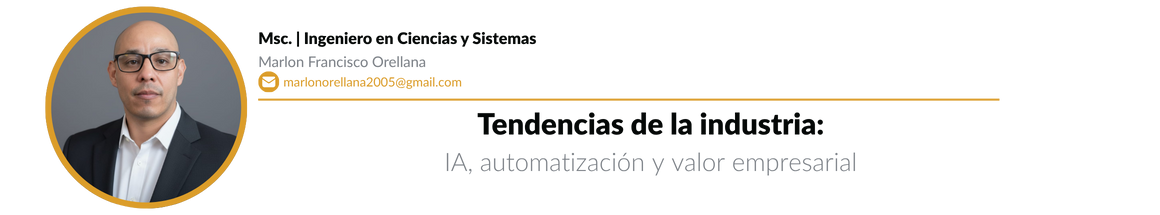
\includegraphics[width=1\linewidth]{autores_seleccionados/e2} \end{center}

\begin {multicols}{2}

\textbf{\emph{YouTube:}} \url{https://youtu.be/OY4QHOD0Vag}

\section{Entrevista}\label{entrevista-1}

\textbf{¿Quién es Marlon Orellana?}

Mi nombre es Marlon Orellana; soy profesor y egresado de la Escuela de Ciencias y Sistemas de la Facultad de Ingeniería de la Universidad de San Carlos de Guatemala (USAC). Como docente, acumulo 18 años de experiencia impartiendo cursos en pregrado y también desarrollo actividades en posgrado.

He sido coordinador de área de la Escuela durante más de cinco años. En ese rol hemos procurado la mejora académica en distintos cursos y temáticas, fortaleciendo la didáctica docente para beneficio del estudiantado. Actualmente soy coordinador del área de Software; tengo a mi cargo cursos que van desde Programación hasta Software Avanzado. Mi objetivo ha sido impulsar una gradación y actualización de conocimientos en beneficio del estudiante.
En el ámbito laboral, he trabajado en empresas internacionales y algunas instituciones nacionales y de gobierno, donde he podido aplicar mis conocimientos, principalmente en compañías con operaciones en Estados Unidos y Europa, con procesos altamente estandarizados. He colaborado, entre otras, con Nielsen, Bayer y ExxonMobil, experiencias que han aportado significativamente a mi formación profesional.

Cuento con tres maestrías: Sistemas, Gestión de Proyectos y Analítica de Datos. Esto me permite desempeñarme en administración de proyectos, analítica de datos y administración de sistemas. Actualmente integro inteligencia artificial en estos tres frentes y exploro la automatización de procesos. En conjunto, estas áreas se entrelazan y generan valor para la empresa en la que trabajo.

He notado un boom en varios temas actuales que me interesa compartir con los estudiantes y profesionales que leen la revista.

\textbf{¿Cómo ve actualmente la industria tecnológica para ingenieros que inician su carrera?}

La industria tecnológica evoluciona muy rápido. Los ciclos de cambio son ya de 12, 6 o incluso 3 meses. Hay gran oferta tecnológica, por lo que el egresado debe elegir ámbitos donde se sienta cómodo y que le agraden para desarrollarse.
Conviene apoyarse en rankings y entidades que evalúan herramientas y tendencias, además de realizar un proceso investigativo propio para tomar decisiones informadas.

\textbf{¿Qué lo motivó a elegir esta profesión?}

Soy Perito Contador y egresé con uno de los mejores promedios de mi institución. Inicialmente me atraían las carreras económicas por tradición familiar, pero, tras analizar el mercado laboral y notar su saturación, opté por mi segunda gran pasión: la tecnología, el hardware y el software. Aunque no tenía bases en física, química, matemática o estadística al nivel requerido, redoblé esfuerzos y lo logré con el apoyo de excelentes catedráticos. Elegí Ingeniería en Ciencias y Sistemas y, hasta hoy, sigo aprendiendo y actualizándome continuamente.

\textbf{¿Cómo fueron sus primeras experiencias laborales?}

A finales de los 2000, la Escuela funcionaba con clases presenciales matutinas, lo que llevaba a que muchos trabajaran hasta el final de la carrera. Empecé, como muchos, en desarrollo en una institución privada; luego pasé al sector público.Observé que en Guatemala la adopción tecnológica iba rezagada por la baja penetración de Internet en aquellos años, mientras empresas internacionales avanzaban con mayor rapidez. Busqué entonces oportunidades en retail y análisis de datos con Nielsen; después pasé a Henkel, lo que me permitió viajar por Centroamérica, Estados Unidos y Alemania, con exposición a estandarización de procesos y analítica para supermercados.

Más tarde llegué a ExxonMobil, una petrolera global, donde crecí mucho profesionalmente. Tras un divest y cierre de operaciones en la región, trabajé temporalmente como Project Manager en un outsourcing tecnológico local para distintos clientes. Luego ingresé a Bayer, donde implementé soluciones para Guatemala y Centroamérica.

Actualmente laboro en Conduent, inicialmente apoyando proyectos del área comercial para grandes clientes ---especialmente en claims del sector salud--- y posteriormente en el área de gobierno (transportación y child support), donde la empresa compite por proyectos tecnológicos para diferentes estados de EE. UU. y Europa. En este entorno aplico gestión de proyectos, analítica de datos y administración de sistemas, además de profundizar en IA y automatización de procesos. Parte de estos aprendizajes los he compartido en congresos estudiantiles, como forma de retribuir al país.

\textbf{¿Qué papel tiene hoy un ingeniero en sistemas en el crecimiento de las empresas tecnológicas?}

El ingeniero en sistemas aporta ahorro de costos, ahorro de tiempo e incremento de calidad mediante tecnología, incluyendo IA. Automatizar procesos repetitivos reduce errores y libera a las personas para tareas de mayor valor. Nuestra misión ---en especial en Guatemala--- es eliminar la operatividad excesiva que desgasta a los equipos. Si no simplificamos procesos y elevamos la calidad, nos ``ahogamos'' en la operación. Automatizar no es ``quitar personal'', sino reorientar talento a actividades estratégicas.

\textbf{¿Qué dificultades tienen los estudiantes al usar tecnologías de aprendizaje vs.~métodos tradicionales?}

El principal reto es adaptarse rápido y usar la tecnología de forma intuitiva. Pero, sobre todo, volver a leer: hoy prevalecen hábitos de consumo rápido y superficial de información. Hace falta lectura comprensiva y profundización para consolidar el aprendizaje.

\textbf{¿Cómo se puede preparar a los estudiantes para usar usar estas tecnologías de forma ética y responsable?}

Se necesitan procesos formativos que dejen clara la responsabilidad en el manejo de datos, información y procesos. Sería valioso incluir, dentro de los cursos o al final de la carrera, módulos o charlas sobre propiedad intelectual, ética profesional y marcos legales/penales aplicables al uso tecnológico (aunque en Guatemala sean aún incipientes, en otros países sí existen). Comprender esto no solo genera buenas prácticas, también evita responsabilidades.

\textbf{¿Qué retos enfrentan los docentes al incluir herramientas de IA en clase?}

Conocer bien las herramientas: alcances, limitaciones, aplicaciones, formas de evaluación y métricas. La diversidad es grande, por lo que hay que identificar si el uso es correcto. También necesitamos apoyo institucional para acortar la curva de aprendizaje docente.

\textbf{¿Cómo medir el verdadero aprendizaje cuando se usa IA?}

Sugiero una aproximación de ``baby steps'': introducir IA gradualmente. En cursos de desarrollo de software, por ejemplo, puede usarse hacia el final en una práctica o componente puntual de un proyecto (p.~ej., detección de rostros, huellas o colores). La IA resuelve una parte, pero el estudiante debe desarrollar el resto. Así, desde cursos básicos se incorporan pequeñas porciones de IA y se escala progresivamente hasta implementaciones más robustas y medibles en cursos avanzados.

\textbf{¿Qué dificultades existen para actualizar planes de estudio e incluir IA?}

La actualización curricular a nivel de carrera es compleja por los procesos de aprobación. Sin embargo, podemos actualizar temáticas dentro de cada curso. Por ejemplo, en Metodologías Ágiles, incorporar herramientas de IA para Scrum, DevOps o gestión visual.
No se trata de ``entregarle el curso a la IA'', sino de usarla como herramienta soportada por conocimiento y lógica. La máquina no debe pensar por nosotros; debemos dominar la base conceptual para enseñar y aprender con criterio.

\textbf{¿Qué acciones universitarias ayudarían a que estas tecnologías mejoren la calidad educativa?}

Desde infraestructura hasta calidad de materiales, recursos y procesos educativos. Sería valioso organizar simposios de discusión sobre IA en educación, modalidad virtual, evaluación justa (mitigando trampas o usos inadecuados de IA), buenas prácticas y políticas.
Referentes como Harvard publican constantemente sobre IA y educación/negocios (el Ing. César Fernández comparte materiales útiles). Hay que investigar, comparar y adoptar buenas prácticas aplicables a nuestro contexto.

\textbf{¿Cómo imagina la evolución del mercado laboral para ingenieros en 5--10 años?}

Un colega asistió a una conferencia de NVIDIA en San Francisco (2025) donde se planteó que el futuro está en el entrenamiento de modelos de IA, más que solo en su uso. Muchos serán usuarios; pocos dominarán el entrenamiento y la profundidad técnica. Comparto esa visión.

\textbf{¿Qué áreas o especializaciones tendrán mayor demanda en el futuro cercano?}

Inteligencia Artificial, automatización de procesos y una analítica de datos potenciada por IA. También el diseño de microprocesadores (chips) ---tema aún incipiente en Guatemala---, y a mediano plazo la computación cuántica.
Transversalmente, la ciberseguridad seguirá siendo clave por la exposición de la información y la necesidad de procesos seguros. Añadiría una capa constante de calidad sobre todos estos temas. Analizar conversaciones en redes sociales y servicios de tendencias también puede orientar sobre qué se está usando.

\textbf{¿Qué lección importante comparte con las nuevas generaciones?}

Como sancarlistas, nuestro gran diferenciador es ser autodidactas: tomar un problema o tecnología desconocida, aprenderla rápido, profundizar, implementar y hacerlo en tiempos cortos.
Aunque enfrentemos limitaciones de aulas o equipo, la actitud y la capacidad de resolver nos vuelven competitivos a nivel técnico. Tal vez falten componentes de análisis económico/financiero, pero técnicamente marcamos diferencia.

\textbf{Mensaje final de Marlon Orellana}

Agradezco a la Escuela, a las autoridades y a ustedes, estudiantes del Consejo Editorial, por este esfuerzo de llevar conocimiento a más personas.Vivimos tiempos donde se valora mucho la inmediatez de las redes; usemos esos canales para difundir conocimiento confiable y útil, en el momento preciso, y motivar la lectura de artículos y revistas.Gracias por el espacio y que las próximas generaciones aporten con fuerza a Guatemala.

\end {multicols}

\medskip

\HRule

\medskip

\chapter{Desarrollo de ciudades inteligentes en la actualidad: tendencias, casos y hoja de ruta para América}\label{ingenerio}

\begin{center}
\includegraphics[width=1\linewidth]{autores_seleccionados/a4} \end{center}

\begin {multicols}{2}

\textbf{\emph{Palabras clave:}} Smart Cities, IoT, Big Data, Gobernanza Digital, Ciberseguridad.

\section{Introducción}\label{introducciuxf3n-3}

En las últimas décadas, el concepto de ciudades inteligentes ha evolucionado de un ideal futurista a una realidad, la alta densidad poblacional en las ciudades de todo el mundo ha llevado a los sectores público y privado a gestionar sistemas complejos en diferentes áreas esenciales como transporte, educación, salud, banca, energía, entre otros. Las nuevas urbes integran tecnologías emergentes como el Internet de las Cosas (IoT), inteligencia artificial (IA), Big Data, ciberseguridad y plataformas en la nube, con el objetivo de optimizar servicios urbanos, mejorar la gobernanza y elevar la calidad de vida de los ciudadanos.

Sin embargo, el camino hacia la consolidación de las ciudades inteligentes no ha sido homogéneo. Mientras Europa y Asia han logrado avances significativos, América Latina enfrenta retos particulares en materia de infraestructura digital, desigualdad y sostenibilidad.

\section{Artículo}\label{artuxedculo-3}

\bigskip

Para la construcción de ciudades inteligentes debemos considerar varios factores y cada ciudad debe ser analizada individualmente podemos considerar los siguiente:

La primera es la consolidación de un IoT obicuo, con sensores desplegados en transporte, energía, salud, seguridad y medio ambiente. Esta capa tecnológica genera datos en tiempo real que permite tomar decisiones informadas.

La segunda tendencia es el uso combinado de IA y Big Data que posibilita la analítica predictiva en movilidad, gestión de emergencias y planificación urbana (Ahad et al.~2023).

La tercera destaca la infraestructura digital avanzada, sustentada con 5G, Edge Computing, y redes definidas por software, que brindan baja latencia y alta confiabilidad(IEEE 2017).

La cuarta tendencia se relaciona con el uso de blockchain y gemelos digitales, tecnologías que ofrecen trazabilidad en trámites y la posibilidad de simular políticas antes de implementarlas.

La quinta tendencia corresponde a la ciberseguridad, entendida como un eje transversal. A medida que se digitalizan los servicios urbanos, crece la superficie de ataque; por ello se requieren arquitecturas Zero Trust, detección temprana de anomalías y talento especializado en defensa digital(AI-Turjman et al.~2025).

La sexta tendencia está vinculada con la sostenibilidad y la inclusión social, factores que aseguren que la tecnología contribuya a reducir brechas y a enfrentar el cambio climático.

Existen casos internacionales ya implementados que refuerzan estas ideas. Barcelona se ha consolidado como pionera en datos abiertos y participación ciudadana; Singapur sobresale en movilidad inteligente y servicios de gobierno digital; Dubái apuesta por la digitalización de trámites con blockchain; mientras que Ámsterdam prioriza la sostenibilidad energética y la colaboración público-privada(Ahad et al.~2023). Estos ejemplos demuestran que no existe un único modelo de ciudad inteligente, sino enfoques que respondan a las particularidades de cada sociedad.

En América Latina, experiencias como las de Medellín con innovación social, Santiago de Chile con transporte eléctrico y ciudad de México con monitoreo ambiental constituyen avances significativos. Sin embargo, la región aún enfrenta limitaciones: desigualdad en el acceso a internet, inseguridad urbana, fragmentación institucional y dependencia de financiamiento externo. Estos retos demandan un enfoque regional y adaptado a las realidades locales.

La hoja de ruta para la región debería contemplar al menos cinco ejes estratégicos:

\begin{itemize}
\tightlist
\item
  El fortalecimiento de infraestructura tecnológica, con prioridad en 5G, fibra óptica y plataformas en la nube con soberanía de datos.
\item
  El diseño de marcos de gobernanza que garanticen, interoperabilidad, protección de datos y apertura de información pública.
\item
  Una política integral de ciberseguridad que incluya centros de respuesta a incidentes y programas de formación.
\item
  La innovación orientada a la sostenibilidad, con energías renovables, blockchain en la gestión de recursos y gemelos digitales para la planificación urbana.
\item
  Eje de inclusión social que asegure la participación ciudadana en la toma de decisiones y reduzca la brecha digital.
\end{itemize}

\bigskip
\bigskip

\section{Conclusiones}\label{conclusiones-3}

El desarrollo de ciudades inteligentes constituye una oportunidad estratégica para la transformar la vida urbana en América Latina. Los avances internacionales demuestran que la clave no radica únicamente en la tecnología, sino en su integración con políticas públicas sólidas y con la participación de la ciudadanía. La región debe avanzar con pasos firmes en cinco dimensiones: infraestructura tecnológica, gobernanza, ciberseguridad, sostenibilidad e inclusión social. Adoptar este enfoque permitirá crear un modelo latinoamericano de ciudad inteligente, capaz de responder a sus desafíos estructurales y aprovechar la innovación para mejorar la calidad de vida de millones de ciudadanos.

\section{Referencias}\label{referencias-3}

\begin{itemize}
\item
  {[}1{]} Ahad, Md Atiqur Rahman, Fadi Al-Turjman, y Rania Kora. ``Smart Cities: IoT Techologies, Big Data, Solutions, Cloud Plataforms, and Cybersecurity Techniques'' Boca Raton: CRC Press, 2024.
\item
  {[}2{]} AI-Turjman, Fadi, et al.~``A Deep Dive into Cybersecurity Solutions for AI-Driven IoT-Enabled Smart Cities in Advanced Communication Networks.'' Computer Communications, 2025.
\item
  {[}3{]} Rodger Lea.``Smart Cities: An Overview of the Technology Trends Driving Smart Cities''. Lancaster University, Marzo,2017.
\end{itemize}

\end {multicols}

\medskip

\chapter{Vibe coding: la frontera entre intuición y programación asistida por IA}\label{pareja6}

\begin{center}
\includegraphics[width=1\linewidth]{autores_seleccionados/a5} \end{center}

\begin {multicols}{2}

\textbf{\emph{Palabras clave:}} Vibe coding, inteligencia artificial, programacion intuitiva, desarrollo ágil, tecnologia.

\section{Introducción}\label{introducciuxf3n-4}

La forma en que entendemos la programación está cambiando rápidamente. Gracias a la inteligencia artificial generativa, crear software ya no depende únicamente de dominar lenguajes de código, sino de interactuar con asistentes capaces de transformar ideas en aplicaciones. Este fenómeno, conocido como vibe coding, convierte la intuición en una herramienta creativa para el
desarrollo tecnológico.{[}1{]}

Lo que antes estaba reservado a expertos en informática, hoy comienza a estar al alcance de cualquier persona con una idea y curiosidad.{[}3{]} Con el progreso acelerado de la inteligencia artificial generativa, ha surgido un nuevo paradigma en el que programar se convierte en un ciclo de retroalimentación entre un usuario y la IA conversacional.{[}2{]}

\section{Artículo}\label{artuxedculo-4}

\bigskip

El término vibe coding se popularizó en febrero de 2025, cuando fue utilizado por primera vez por Andrej Karpathy, cofundador de OpenAI, en referencia a esta forma intuitiva y experimental de crear aplicaciones. {[}2{]} A diferencia del enfoque tradicional, donde aprender lenguajes de programación era indispensable, el vibe coding se apoya en la inteligencia artificial para que el usuario interactúe de manera intuitiva, casi como si hablara con un asistente personal.

Lo más llamativo de esta nueva forma de programar es su capacidad para democratizar el acceso a la creación tecnológica. {[}1{]} Hoy basta con tener una idea y traducirla en instrucciones simples para que una IA genere aplicaciones funcionales. Este cambio recuerda cómo los lenguajes de alto nivel
hicieron más accesible la informática, pero ahora llevado al siguiente nivel.{[}3{]}

Este enfoque se adapta perfectamente a los marcos de desarrollo ágil.{[}2{]} La premisa de ``probar primero y refinar después'' permite acelerar la entrega de resultados y fomenta la experimentación.{[}2{]}

La inteligencia artificial puede generar código útil, pero también es susceptible a errores o vulnerabilidades de seguridad. ¹ La supervisión humana sigue siendo crucial, ya que el juicio y el contexto que aporta una persona son insustituibles.{[}1{]}

\begin {flushleft}
\noindent\begin{minipage}[c]{\columnwidth}

\begin{center}
\includegraphics[width=1\linewidth]{imagenes_articulos_seleccionados/A5/p1} \end{center}
\figcaption{Ventajas y desafíos del vibe coding.}

\end{minipage}
\end {flushleft}

Como se observa en la Figura 6.1, el vibe coding presenta un balance entre oportunidades y retos que deben ser gestionados cuidadosamente para maximizar su efectividad en el desarrollo de software.

\bigskip

\textbf{Caso de aplicación}
Un ejemplo representativo es el artículo publicado en WIRED España, donde se exponen casos de personas sin conocimientos técnicos que lograron crear aplicaciones para resolver problemas cotidianos. {[}4{]} Estos casos muestran que el vibe coding no es solo una curiosidad tecnológica, sino un cambio cultural que redefine lo que significa programar en la era de la inteligencia artificial.

\bigskip
\bigskip

\section{Conclusiones}\label{conclusiones-4}

El desarrollo de ciudades inteligentes constituye una oportunidad estratégica para la transformar la vida urbana en América Latina. Los avances internacionales demuestran que la clave no radica únicamente en la tecnología, sino en su integración con políticas públicas sólidas y con la participación de la ciudadanía. La región debe avanzar con pasos firmes en cinco dimensiones: infraestructura tecnológica, gobernanza, ciberseguridad, sostenibilidad e inclusión social. Adoptar este enfoque permitirá crear un modelo latinoamericano de ciudad inteligente, capaz de responder a sus desafíos estructurales y aprovechar la innovación para mejorar la calidad de vida de millones de ciudadanos.

\section{Referencias}\label{referencias-4}

\begin{itemize}
\item
  {[}1{]} Harkar, Shalini. ``What Is Vibe Coding?'' IBM Think, Abril,2025 . Accedido el 22 de agosto de 2025.\href{https://www.ibm.com/think/topics/vibe-coding.}{https://www.ibm.com}.
\item
  {[}2{]} Indiano, Andrea. ``Ya se puede crear software sin saber programar.'' Campus Technology, Marzo,2025. Accedido el 22 de agosto de 2025. \href{https://es.wired.com/articulos/ya-se-puede-crear-software-sin-saber-programar}{https://es.wired.com}
\item
  {[}3{]} Khan, Tasmiha, y Amanda Downie.''What Is No-Code?{}``. IBM Think,2025. Accedido el 16 de agosto de 2025. \href{https://www.ibm.com/think/topics/no-code}{https://www.ibm.com}
\item
  {[}4{]} Kumar, Madhukar.''A Comprehensive Guide to Vibe Coding Tools.''. Medium
  (Software, AI and Marketing), Marzo,2025. Accedido el 3 de agosto de 2025. \href{https://medium.com/madhukarkumar/a-comprehensive-guide-to-vibe-coding-tools2bd35e2d7b4f}{https://www.medium.com}
\end{itemize}

\end {multicols}

\medskip

\chapter{El paradigma de Svelte: menos código, más rendimiento}\label{pareja48}

\begin{center}
\includegraphics[width=1\linewidth]{autores_seleccionados/a6} \end{center}

\begin {multicols}{2}

\textbf{\emph{Palabras clave:}} Framework, Frontend, Svelte, Rendimiento, Web, JavaScript.

\section{Introducción}\label{introducciuxf3n-5}

Actualmente, las aplicaciones son cada vez más pesadas, teniendo una mayor complejidad de código y necesidad de mejorar la experiencia de usuario. Es por ello que, en los últimos años, Svelte, un nuevo framework frontend de JavaScript, salió a la luz ganando terreno con su paradigma de compilador que genera JavaScript puro de una forma altamente optimizada, planteando una filosofía distinta: menos código, más rendimiento.

Grandes empresas como Apple Music, Spotify y The New York Times ya utilizan Svelte en sus proyectos para mejorar la experiencia de usuario y optimizar el rendimiento. A pesar de que React siga siendo el preferido en el mercado laboral, Svelte ha comenzado a destacarse por su simplicidad, menor consumo de recursos, tiempos de carga más rápidos, código final mucho más ligero y una documentación superior, reduciendo así la curva de aprendizaje.

\section{Artículo}\label{artuxedculo-5}

\bigskip

\textbf{¿Qué hace diferente a Svelte?}

Según Mozilla (2025) la principal diferencia de Svelte frente a React o Vue es su compilador, el cual devuelve HTML, CSS y JavaScript puro optimizado durante el tiempo de construcción, eliminando la necesidad de interpretar código en tiempo de ejecución. El resultado final es código JavaScript que interactúa directamente con el DOM. Esto se traduce en un menor consumo de recursos y tiempos de carga más rápidos.

Otra de las diferencias de Svelte radica en la ausencia de un DOM virtual, lo que le permite ahorrar una sobrecarga significativa de trabajo, ya que el código de JavaScript generado interactúa directamente con el DOM real. Esto lo diferencia de frameworks como React, que utilizan un DOM virtual que luego es traducido a un DOM real (Mozilla 2025).

Asimismo, la arquitectura de Svelte ofrece ventajas significativas, como una reducción
sustancial en la cantidad de líneas de código, entre un 30\% y un 40\% menos en comparación
con React, lo que favorece una mejor legibilidad gracias a una sintaxis similar a HTML, CSS
y JavaScript puro, disminuyendo así su curva de aprendizaje (Bhushan 2025).

\bigskip

\textbf{Una nueva forma de pensar el rendimiento}
Se han realizado varios estudios que demuestran que Svelte representa una nueva forma de pensar el rendimiento al ofrecer grandes ventajas en velocidad, optimización y eficiencia. Uno de los estudios más recientes es el de Putra et al.~(2025) quienes demostraron que Svelte logra tiempos de renderizado un 35\% más rápidos que React, tamaños de bundle más reducidos y un uso de memoria más eficiente, superando a React y Vue en todas las métricas evaluadas.

Asimismo, otra de las investigaciones sobre la manipulación del DOM y el consumo de memoria en Svelte fue realizada por Dékány (2025) en la Universidad de Masaryk, concluyendo que existe una reducción significativa de la latencia en la interacción y una mejora de la escalabilidad en entornos de alta demanda al usar JavaScript nativo optimizado. Esto marca un cambio de paradigma respecto a los frameworks tradicionales.

\bigskip

\textbf{Menos código: simplicidad y reactividad}
Según Bhushan (2025) una de las mayores virtudes de Svelte radica en su capacidad para lograr una sintaxis clara y concisa, lo que se traduce directamente en un menor uso de código al momento de implementar funcionalidades en comparación con otros frameworks. Asimismo, Svelte elimina casi por completo la necesidad de importaciones de hooks, gestionando la reactividad mediante JavaScript estándar. Es ``JavaScript con superpoderes''.

\bigskip

\textbf{Adopción en la industria}
Svelte ha experimentado un crecimiento significativo en adopción empresarial desde su versión 3 en 2019. Actualmente cuenta con más de 60,000 estrellas en su repositorio de GitHub, lo que refleja una gran lealtad y satisfacción por parte de los desarrolladores que lo utilizan. A continuación, se presenta una gráfica de popularidad de Svelte en los últimos años.

\begin {flushleft}
\noindent\begin{minipage}[c]{\columnwidth}

\begin{center}
\includegraphics[width=1\linewidth]{imagenes_articulos_seleccionados/A6/p1} \end{center}
\figcaption{Popularidad Frameworks Frontend. En Github}

\end{minipage}
\end {flushleft}

La gráfica de popularidad de frameworks frontend muestra el dominio sostenido de React, aunque con una leve caída desde su pico en 2020/2021; Angular y Vue también presentan descensos, mientras que Svelte destaca como el de mayor crecimiento desde 2020. No obstante, al ser un framework relativamente nuevo, su ecosistema aún es reducido en comparación con sus competidores, lo que se traduce en una menor demanda laboral y mercado más reducido.

\bigskip
\bigskip

\section{Conclusiones}\label{conclusiones-5}

Svelte se presenta como un paradigma innovador en el desarrollo frontend al combinar simplicidad y rendimiento mediante un modelo de compilación que produce código nativo optimizado, con claras ventajas frente a frameworks como React. Las investigaciones señalan mejoras en tiempos de renderizado, eficiencia en el uso de memoria y escalabilidad, lo que lo convierte en una opción atractiva para proyectos que requieren rapidez y estabilidad. Su
sintaxis clara y la reducción de líneas de código facilitan la legibilidad y el proceso de aprendizaje de los desarrolladores. No obstante, la demanda laboral de Svelte aún es reducida en comparación con la de sus competidores, existiendo la necesidad de fortalecer su comunidad de desarrollo. Finalmente, queda abierta la discusión sobre si este enfoque logrará consolidarse como un estándar predominante en la industria tecnológica global en los próximos años.

\section{Referencias}\label{referencias-5}

\begin{itemize}
\item
  {[}1{]} Bhushan, Ashirvad. ``Svelte vs.~React: características, rendimiento y más.'' Kinsta, Enero,2025 . Accedido el 17 de agosto de 2025.\\
  \href{https://kinsta.com/es/blog/svelte-vs-react/.}{https://kinsta.com/}.
\item
  {[}2{]} Dékány, Martin. ``Comparative Analysis of React, Vue.js, and Svelte.'' tesis de licenciatura,Universidad de Masaryk,2025. (tesis de licenciatura,
  Universidad de Masaryk, 2025), 45. \href{https://is.muni.cz/th/gjz8s/thesis.pdf}{https://is.muni.cz}
\item
  {[}3{]} Mozilla.``Introducción a Svelte - Aprende desarrollo web.'' MDN Web Docs, 2025. Accedido 13 de agosto de 2025.\\
  \href{https://developer.mozilla.org/es/docs/Learn_web_development/Core/Frameworks_libraries/Svelte_getting_started.}{https://www.developer.mozilla.org}
\item
  {[}4{]} Putra, Fauzan Prasetyo Eka, Hasbullah, Farhan Muslim, y Reni Paradina.``Technical Performance Comparison of Modern Frontend Frameworks - Study on Svelte, React, and Vue.'', 2025. Brilliance: Research of Artificial Intelligence 5, no. 1: 355--364. DOI: 10.47709/brilliance.v5i1.6133.
\item
  {[}5{]} Krotoff,Tanguy.``Popularidad de frameworks frontend.'',GitHub Gist,Marzo, 2025. Accedido 12 de
  agosto de 2025. \href{https://gist.github.com/tkrotoff/b1caa4c3a185629299ec234d2314e190.}{https://gist.github.com}
\end{itemize}

\end {multicols}

\medskip

\SectionPDF{images/seccion3.pdf}{32}

\chapter{¿Desarrollador junior y sin experiencia? La batalla del primer empleo}\label{pareja29}

\begin{center}
\includegraphics[width=1\linewidth]{autores_seleccionados/a7} \end{center}

\begin {multicols}{2}

\textbf{\emph{Palabras clave:}} Junior, desarrollador, empleo, tecnología, experiencia.

\section{Introducción}\label{introducciuxf3n-6}

Quien se enfrenta al primer empleo como desarrollador descubre muy pronto que ``junior'' no siempre significa ``principiante''. Los portales están llenos de vacantes que piden varios años de experiencia, las entrevistas técnicas recuerdan más a competencias de programación que a lo que generalmente se aprende en los cursos universitarios.

Detrás de esta pared inicial de requisitos contradictorios, existe un camino: perseverancia,autodidactismo y, a veces, un golpe de suerte, pueden abrir esa primera puerta. Pero el desafío no termina al recibir la oferta, es ahí donde comienza la verdadera prueba de fuego: demostrar la capacidad voraz de aprender y adaptarse al ritmo abrumador del mundo laboral real.

\section{Artículo}\label{artuxedculo-6}

\bigskip

\textbf{La paradoja de la experiencia necesaria}

Alex apagó su computadora con un suspiro. Su bandeja de entrada era un monumento al rechazo en la mayoría de sus solicitudes laborales.Su actual crimen, ser un recién graduado en la licenciatura en Ingeniería en Ciencias y
Sistemas en un mundo que pide guerreros veteranos para puestos de novato.

Su caso no es aislado, es la norma. Un análisis de vacantes revela la paradoja: una gran parte de las ofertas para desarrolladores junior exigen entre 1 y 3 años de experiencia laboral previa{[}1{]}, algo paradójico para quienes buscan su primera oportunidad.

\bigskip

\textbf{El muro de la entrevista técnica}

En las entrevistas, el choque era palpable. En la universidad había aprendido a resolver problemas abstractos, y algoritmos complejos. Y lo hacía bien. Pero en su primera entrevista técnica, el interrogatorio era distinto: ``¿Has
trabajado con algún framework de persistencia como Hibernate o JPA?'', ``¿Has participado en algún proyecto usando metodologías ágiles como Scrum?''.

Alex balbuceó respuestas teóricas, y solo pensaba que en la universidad se habían centrado en desarrollar los cimientos, no en las herramientas del día a día. La siguiente tabla muestra una comparación entre las habilidades y conocimientos que se enseñan en la universidad versus lo que exige el mercado laboral.

\begin {flushleft}
\noindent\begin{minipage}[c]{\columnwidth}

\begin{center}
\includegraphics[width=1\linewidth]{imagenes_articulos_seleccionados/A7/p1} \end{center}
\figcaption{Comparativa vs Mercado Laboral.}

\end{minipage}
\end {flushleft}

\bigskip

\textbf{Un mercado laboral implacable}

El contexto no ayudaba. Con oleadas de despidos en tech,
la competencia se había multiplicado{[}2{]}. Alex ya no solo rivalizaba con recién graduados, sino con desarrolladores con 2 o 3 años de experiencia dispuestos a aceptar puestos junior con tal de reinsertarse. Cada ``No'' golpeaba su moral. ``¿Y si no estoy hecho para esto?'', pensaba. Estaba a punto de rendirse cuando llegó un email diferente: ``Invitación a entrevista final''.

\bigskip

\textbf{La oportunidad: una filosofía diferente.}

La entrevista fue diferente desde el inicio. En lugar de un interrogatorio técnico agresivo, fue una conversación honesta sobre su proyecto de grado, su lógica para resolver problemas y su voluntad de aprender. El CTO del startup le explicó: ``Aquí no buscamos bibliotecas andantes, buscamos mentes curiosas. Las tecnologías las puedes aprender; las ganas, no''. Esa filosofía fue el boleto de entrada que Alex necesitaba. Firmó su contrato con una mezcla de euforia y alivio, creyendo que la parte más difícil había terminado.

Lo que parecía el final del camino era apenas el inicio de una nueva batalla. Alex pasó de un ``Hola mundo'' universitario a enfrentarse con repositorios gigantes, microservicios y despliegues que parecían otro idioma. El síndrome del impostor apareció rápido: ``¿Y si fue un error contratarme?''. Ahí entendió que programar es solo la mitad del reto; la otra mitad es trabajar en equipo, pedir ayuda y aprender a moverse en un mundo donde las tecnologías cambian todo el tiempo.

Al inicio fue agotador: noches de tutoriales, errores y dudas. Pero con cada paso, Alex descubrió algo clave: no importa saberlo todo, importa la actitud. Cada fallo se volvió una lección y cada pequeño logro, un triunfo. Lo que antes parecía imposible como usar Git o Docker terminó siendo parte de su caja de herramientas. El primer empleo no es el final del camino, es el inicio del verdadero aprendizaje. Y aunque la lucha es dura, también es la etapa donde más se crece.

\bigskip
\bigskip

\section{Conclusiones}\label{conclusiones-6}

El caso de Alex refleja la dualidad del primer empleo como desarrollador: la batalla por conseguirlo y la lucha aún más dura por mantenerlo. Lo que inicia como frustración ante los rechazos se transforma en incertidumbre frente al desconocimiento, y poco después, en una carrera de aprendizaje acelerado. El verdadero valor de un junior no está en dominar todas las tecnologías desde el primer día, sino en su capacidad de adaptarse, preguntar y crecer en medio de la presión. Cada error se convierte en un peldaño, cada corrección en un paso hacia la madurez profesional. El camino del primer empleo está lleno de dudas, pero también de descubrimientos que ningún libro enseña. Para quienes apenas comienzan, la lección es clara: no se trata de evitar la batalla, sino de aprender a pelearla con paciencia, disciplina y resiliencia. Porque el primer empleo no es la meta, es apenas el inicio del viaje.

\section{Referencias}\label{referencias-6}

\begin{itemize}
\item
  {[}1{]} Codica. ``Qué exigen los empleadores a los junior: análisis de vacantes para programadores junior.'' Academia de programadores en línea. Accedido el 18 de agosto de 2025. \href{https://codica.la/blog/que-exigen-los-empleadores-a-los-junior-analisis-de-vacantes}{https://codica.la}.
\item
  {[}2{]} United Code, ``When Will the Tech Job Market Recover? 2025 Hiring Outlook, Layoffs,and Policy Shifts.'' United Code, 2025. Accedido el 19 de agosto de 2025. \href{https://unitedcode.net/when-will-the-tech-job-market-recover-2025-hiring-outlook-layoffsand-policy-shifts/?_x_tr_sl&_x_tr_tl&_x_tr_hl}{https://unitedcode.net}
\item
  {[}3{]} 4GeeksAcademy.``Síndrome del Impostor: El peor enemigo de todo programador junior'' 4GeeksAcademy. Accedido el 20 de agosto de 2025. \href{https://4geeksacademy.com/es/tendencias-y-tecnologia/sindrome-del-impostor}{https://www.4geeksacademy.com}
\item
  {[}4{]} Stack Overflow.``2024 Developer Survey: Key Insights.'' Stack Overflow Research, 2024. Accedido el 20 de agosto de 2025.\\
  \href{https://survey.stackoverflow.co/2024}{https://www.survey.stackoverflow.co}
\end{itemize}

\end {multicols}

\medskip

\chapter{Carreras en tecnología: diferencias y aprendizajes entre startups y grandes corporaciones}\label{pareja30}

\begin{center}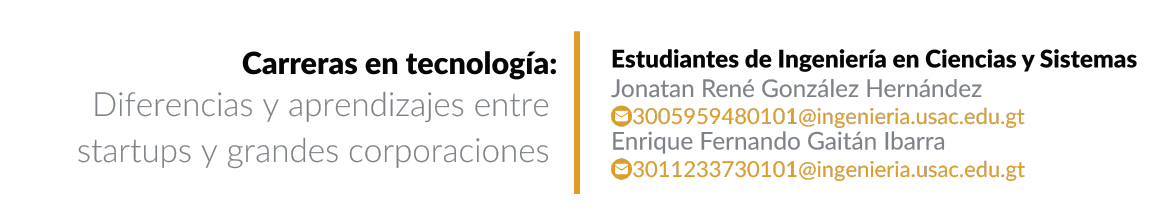
\includegraphics[width=1\linewidth]{autores_seleccionados/a8} \end{center}

\begin {multicols}{2}

\textbf{\emph{Palabras clave:}} Startups, grandes empresas, trabajo, industria tecnológica, oportunidades.

\section{Introducción}\label{introducciuxf3n-7}

En el ecosistema tecnológico conviven desde startups de unas pocas personas hasta corporaciones globales con decenas de miles de empleados. La experiencia laboral varía de manera notable según el tamaño de la organización: estabilidad y beneficios, cultura, ritmo de trabajo, aprendizaje, crecimiento profesional y redes de contacto se experimentan de forma distinta en cada contexto.

En Guatemala y América Latina, donde predominan las PYMES, muchas trayectorias comienzan en empresas pequeñas; mientras que en Estados Unidos abundan las grandes tecnológicas con estructuras formales y paquetes de compensación más robustos. Este artículo compara, con un enfoque práctico, las diferencias más relevantes entre ambos mundos para orientar a estudiantes y profesionales en la elección de sus caminos de desarrollo profesional.

\section{Artículo}\label{artuxedculo-7}

\bigskip

\textbf{Comparativa}
\textbf{Estabilidad económica y beneficios}

Las corporaciones grandes suelen sostener mejores salarios, seguros médicos, bonos y planes de retiro, lo que permite planificar una carrera a largo plazo. En Guatemala y la región, además, el empleo en pequeñas empresas suele venir con mayores brechas salariales y menor protección social, lo que refuerza la percepción de estabilidad cuando se accede a organizaciones de mayor tamaño.{[}1{]}

En el otro extremo, muchas startups operan con presupuestos ajustados: pueden pagar menos al inicio y ofrecer participación accionaria como apuesta de alto riesgo/alto retorno si la empresa crece.{[}2{]}

\bigskip

\textbf{Cultura y modo de trabajo}

En compañías grandes predominan procesos definidos, jerarquías claras y coordinación entre múltiples equipos. Esto garantiza orden, pero puede traducirse en burocracia y ciclos de decisión más lentos.{[}3{]}En empresas pequeñas la comunicación es directa, las ideas se prueban rápido y el impacto individual se percibe de inmediato; ese dinamismo y cercanía con los fundadores crea sentido de pertenencia, aunque con menos estructura formal para guiar el crecimiento.{[}2{]}

\begin {flushleft}
\noindent\begin{minipage}[c]{\columnwidth}

\begin{center}
\includegraphics[width=1\linewidth]{imagenes_articulos_seleccionados/A8/p1} \end{center}
\figcaption{ Comparativa entre empresas pequeñas y grandes en estabilidad, cultura, ritmo de trabajo, aprendizaje y networking.}

\end{minipage}
\end {flushleft}

\bigskip

\textbf{Desarrollo Profesional}

Los grandes empleadores ofrecen rutas de carrera estructuradas (junior--senior--lead--manager), evaluaciones periódicas y formación formal; el avance puede ser más lento, pero consistente y con prestigio de marca. En empresas pequeñas, la exposición es versátil: una persona puede liderar en poco tiempo, asumir decisiones técnicas y de producto y entender el negocio de punta a punta; el aprendizaje es intenso y práctico, aunque dependa menos de programas formales y más del día a día.

\bigskip
\bigskip

\section{Conclusiones}\label{conclusiones-7}

No existe una respuesta universal sobre ``qué es mejor''. Las empresas grandes ofrecen estabilidad, compensación y rutas de carrera claras, aunque pueden sentirse más lentas y especializadas. Las startups brindan aprendizaje acelerado, impacto visible y rápido crecimiento en responsabilidades, aunque con mayor riesgo y presión operativa. Para un perfil en formación, una estrategia útil es combinar experiencias: iniciar en una empresa pequeña
para ganar versatilidad y luego vivir la escala y el rigor de una organización grande. Así se capitaliza lo mejor de ambos mundos: innovación y adaptabilidad, junto con estructura y proyección internacional. Al final, lo importante no es el tamaño de la empresa, sino la forma en que cada entorno se ajusta a las metas personales y profesionales, permitiendo construir una trayectoria sólida y flexible en el cambiante ecosistema tecnológico.

\section{Referencias}\label{referencias-7}

\begin{itemize}
\item
  {[}1{]} Organización Internacional del Trabajo (OIT). ``, Panorama Laboral Temático. Pequeñas empresas, grandes brechas: Empleo y condiciones de trabajo en las MYPE de América Latina y el Caribe'' Lima: OIT, 2015. \href{https://www.ilo.org/sites/default/files/wcmsp5/groups/public/\%40americas/\%40ro-lima/documents/publication/wcms_398103.pdf}{https://ilo.org}.
\item
  {[}2{]} Orosz,Gergely. ``Working at a Startup vs in Big Tech'' The Pragmatic Engineer, Septiembre,2023. \href{https://blog.pragmaticengineer.com/working-at-a-startup-vs-in-big-tech/}{https://blog.pragmaticengineer.com}
\item
  {[}3{]} Equipo HR Connect.``¿Es mejor trabajar en una gran empresa o en una startup?''. HR Connect, s. f, Abril,2025. Accedido el 9 de abril de 2025. \href{https://www.hrconnect.cl/desarrollo/es-mejor-trabajar-en-una-gran-empresa-o-en-una-startup/}{https://www.hrconnect.cl/}
\end{itemize}

\end {multicols}

\medskip

\chapter{De la universidad al mundo laboral: lo que las empresas esperan de ti}\label{pareja31}

\begin{center}
\includegraphics[width=1\linewidth]{autores_seleccionados/a9} \end{center}

\begin {multicols}{2}

\textbf{\emph{Palabras clave:}} mercado laboral, recién egresado, empleabilidad, innovación.

\section{Introducción}\label{introducciuxf3n-8}

En un mundo donde la tecnología avanza con rapidez, la ingeniería en sistemas se perfila como una de las carreras con mayor proyección. La digitalización de sectores productivos, la automatización de procesos y la innovación han incrementado la demanda de profesionales capaces de diseñar e implementar soluciones tecnológicas eficientes, convirtiendo a estos ingenieros en actores clave del desarrollo empresarial.

Ante este panorama surge una pregunta esencial: ¿qué espera el mercado laboral de un ingeniero en sistemas recién egresado? Más allá de las bases en programación, redes y bases de datos, las empresas buscan un perfil integral que combine conocimientos técnicos, experiencia práctica, habilidades blandas y mentalidad innovadora para afrontar los retos de la transformación digital.

\section{Artículo}\label{artuxedculo-8}

\bigskip

\textbf{Alta demanda laboral y versatilidad profesional}

La carrera de ingeniería en sistemas es altamente demandada a nivel global. Los recién egresados encuentran oportunidades en sectores como salud, finanzas, educación, manufactura y comercio electrónico. Esta versatilidad implica que los profesionales deben adaptarse a distintos entornos, comprender las necesidades específicas de cada industria y traducirlas en soluciones tecnológicas efectivas (Valacich y Schneider 2021).

\textbf{Competencias técnicas clave}
Los egresados deben dominar fundamentos de programación, bases de datos, arquitectura de software y redes. Sin embargo, el mercado actual valora también conocimientos en metodologías ágiles, ciberseguridad y tecnologías emergentes como inteligencia artificial, cómputo en la nube, análisis de datos e Internet de las Cosas (IoT). No se espera que sean expertos en todo, pero sí que tengan capacidad de aprendizaje continuo (Pressman y Maxim 2019).

\textbf{Habilidades blandas como diferenciador}
Las empresas reconocen que el éxito no depende únicamente de lo técnico. La comunicación efectiva, el trabajo en equipo, la resolución de problemas y la adaptabilidad son competencias esenciales. Un recién egresado que pueda transmitir ideas con claridad y colaborar en equipos multidisciplinarios tendrá una ventaja competitiva (Marr 2021).

\textbf{Innovación y mentalidad de crecimiento}
El mercado percibe a los jóvenes ingenieros como agentes de innovación. Se espera que aporten ideas frescas, cuestionen procesos tradicionales y propongan soluciones creativas. Aquellos con una mentalidad de crecimiento y disposición para aprender y mejorar constantemente encuentran mayores oportunidades de destacar en sus roles (Valacich y Schneider 2021).

\textbf{Competencias técnicas vs.~habilidades blandas}
A continuación, se presenta una tabla comparativa que sintetiza las principales competencias que las empresas valoran en un ingeniero en sistemas recién egresado.

\begin {flushleft}
\noindent\begin{minipage}[c]{\columnwidth}

\begin{center}
\includegraphics[width=1\linewidth]{imagenes_articulos_seleccionados/A9/p1} \end{center}
\figcaption{Competencias técnicas y habilidades blandas en ingenieros en sistemas.}

\end{minipage}
\end {flushleft}

\bigskip
\bigskip

\section{Conclusiones}\label{conclusiones-8}

El mercado laboral para los ingenieros en sistemas recién egresados exige un perfil integral que combine conocimientos técnicos sólidos, habilidades blandas y una mentalidad innovadora. Mientras que la programación, las bases de datos y las redes constituyen la base técnica, la comunicación, el trabajo en equipo y la adaptabilidad son determinantes para la integración en entornos profesionales. Asimismo, la experiencia práctica y la disposición para aprender constantemente permiten que los jóvenes egresados enfrenten con éxito los retos del mundo laboral. En este contexto, quienes logran unir lo técnico con lo interpersonal e innovador se convierten en profesionales competitivos capaces de generar valor y liderar la transformación digital de las organizaciones, asegurando así un crecimiento sostenido en su carrera profesional.

\section{Referencias}\label{referencias-8}

\begin{itemize}
\item
  {[}1{]} Laudon, Kenneth C., y Jane P. Laudon. Sistemas de información gerenciales. 16ª ed.~México: Pearson, 2020.
\item
  {[}2{]} Marr, Bernard. Tecnología e innovación en la empresa digital. Londres: Kogan Page, 2021.
\item
  {[}3{]} Pressman, Roger S., y Bruce R. Maxim. Ingeniería de software: un enfoque práctico. 9ª ed.~México: McGraw-Hill, 2019.
\item
  {[}4{]} Valacich, Joseph S., y Christoph Schneider. Information Systems Today: Managing in the Digital World. 9ª ed.~México: Pearson, 2021.
\end{itemize}

\end {multicols}

\medskip

\SectionPDF{images/seccion4.pdf}{37}

\chapter{El juramento ético de la tecnología: la promesa pendiente que falta en la ingeniería de software}\label{pareja13}

\begin{center}
\includegraphics[width=1\linewidth]{autores_seleccionados/a10} \end{center}

\begin {multicols}{2}

\textbf{\emph{Palabras clave:}} Compromiso, Ética, Responsabilidad, Juramento, Inteligencia artificial.

\section{Introducción}\label{introducciuxf3n-9}

En la actualidad, los ingenieros de software tienen en sus manos una responsabilidad que trasciende la escritura de código. El mal manejo de sistemas puede provocar filtraciones de datos personales, vulneración de cuentas y pérdidas millonarias, afectando la confianza y seguridad de millones de usuarios. Y además pueden tener repercusiones legales y éticas significativas.

Así como los médicos realizan un juramento que compromete su labor con la vida y el bienestar humano, surge la pregunta: ¿deberían los desarrolladores de software asumir también un compromiso ético formal? No se trata solo de la parte técnica del desarrollo, sino también de la responsabilidad moral que tienen quienes crean el software que sostiene gran parte de la vida moderna.

\section{Artículo}\label{artuxedculo-9}

\bigskip

Existen intentos formales de guiar la responsabilidad de los ingenieros de software mediante códigos éticos. Organizaciones como la Association for Computing Machinery (ACM) y el IEEE Computer Society han establecido lineamientos que destacan valores fundamentales como la privacidad, la seguridad, la honestidad y la responsabilidad social en la creación de tecnología.

De hecho, en 1997 se presentó el Software Engineering Code of Ethics, concebido como un marco de principios que funciona de manera similar a un juramento profesional{[}3{]}. Sin embargo, estos códigos carecen de obligatoriedad, rara vez son exigidos por las empresas y no cuentan con mecanismos de supervisión legal, lo que los convierte en recomendaciones más que en compromisos vinculantes, dejando la ética en manos de la conciencia individual de cada ingeniero.

En Guatemala y en gran parte de la región, estos códigos no se aplican de manera efectiva principalmente porque no existe una regulación específica que obligue a los ingenieros de software a cumplir con un juramento ético, lo que hace que la aplicación de principios propuestos por la ACM o el IEEE sea irregular y dependa de la madurez de cada organización. A diferencia de profesiones como la medicina o la abogacía, donde los colegios profesionales ejercen control, en la tecnología no hay una entidad que fiscalice la práctica.

\begin {flushleft}
\noindent\begin{minipage}[c]{\columnwidth}

\begin{center}
\includegraphics[width=1\linewidth]{imagenes_articulos_seleccionados/A10/p1} \end{center}
\figcaption{Países afectados por el caso de Cambridge Analytica.}

\end{minipage}
\end {flushleft}

\bigskip

\textbf{La inteligencia artificial como una herramienta para la personalización}

Un ejemplo bastante claro sobre ignorar los códigos éticos y la falta de responsabilidad en el mundo tecnológico es el caso de Cambridge Analytica, consultora de la campaña electoral del presidente Donald Trump, obtuvo datos sin el consentimiento de millones de usuarios para influir en el proceso electoral de los Estados Unidos{[}2{]}. Solo en este país 70,632,350 usuarios
(ver fig.~12.1) fueron afectados por el escándalo de Cambridge Analytica, lo que evidenció la importancia de establecer límites sobre el uso de datos en el mundo digital.

En el mundo IT la ética es un tema amplio y complejo, cada avance o cambio tecnológico introduce nuevos retos éticos, el ejemplo más reciente es la llegada de la inteligencia artificial{[}1{]}. La IA ha traído consigo una nueva serie de preocupaciones éticas, exigiendo que individuos y organizaciones se replanteen el marco de decisiones dentro de lo que se considera o no ético. Exponiendo la necesidad de atender de forma responsable las decisiones digitales de las tecnologías de la información.

Hay dos puntos éticos principales que se deben considerar con la adopción y el uso de la inteligencia artificial:

\begin{itemize}
\item
  Los algoritmos no son neutrales: La inteligencia artificial se entrena con información histórica, por lo que puede presentar sesgos basados en datos históricos de épocas pasadas. También puede presentar sesgos derivados de creencias o preferencias políticas, religiosas, culturales de quién sea dueño de los algoritmos de IA.
\item
  Precisión en las decisiones basadas en IA: Con la adopción de la inteligencia artificial por individuos y organizaciones, cada vez son más quienes toman decisiones basadas en inteligencia artificial, pero es importante considerar que la IA está entrenada con información que puede llegar a ser inexacta o puede estar manipulada para responder a intereses particulares, influyendo en las recomendaciones o respuestas ofrecidas por
  la misma.
\end{itemize}

\bigskip
\bigskip

\section{Conclusiones}\label{conclusiones-9}

Aunque existen códigos de ética para la ingeniería de software, su aplicación aún sigue siendo más aspiracional que real, limitada por la falta de regulación y la influencia de intereses corporativos y gubernamentales. Esta realidad se hace evidente en numerosos países, donde además surgen nuevos desafíos vinculados a la inteligencia artificial, cuyo entrenamiento puede responder a los intereses de quienes controlan y financian sus algoritmos. A esto se suma el diseño de algoritmos de redes sociales que fomentan la adicción, priorizando la rentabilidad sobre el bienestar humano. Un juramento ético permitiría recordar que cada línea de código puede influir en millones de vidas y que la responsabilidad del ingeniero no se limita a entregar un producto funcional, sino a garantizar que la tecnología sirva al bien común y no a intereses particulares.

\section{Referencias}\label{referencias-9}

\begin{itemize}
\item
  {[}1{]} Dauchess, Alexandra.``\,``Understanding the Importance of Ethics in Information Technology''. Marymont University (blog). Accedido el 15 de agosto de 2025. \href{https://marymount.edu/blog/understanding-the-importance-of-ethics-in-information-technology/}{https://marymount.edu}.
\item
  {[}2{]} Fundación Fepropaz. ``La ética en el desarrollo de tecnología: retos para las nuevas generaciones'' Fundación Fepropaz,16 de diciembre de 2024. \href{https://fepropaz.com/etica-y-tech/}{https://fepropaz.com}
\item
  {[}3{]} Gotterbarn, Don, Miller Keith, y Simon Rogerson.``\,``Software engineering code of ethics''. Communications of the ACM 40, no. 11 (noviembre de 1997): 110--118. \href{https://www.doi.org\%5Dhttps://doi.org/10.1145/265684.265699}{https://www.doi.org}
\end{itemize}

\end {multicols}

\medskip

\chapter{Un riesgo oculto en la era digital: Síndrome del túnel carpiano.}\label{medico}

\begin{center}
\includegraphics[width=1\linewidth]{autores_seleccionados/a11} \end{center}

\begin {multicols}{2}

\textbf{\emph{Palabras clave:}} salud mental, salud física, síndrome del túnel carpiano, ergonomía personalizada.

\section{Introducción}\label{introducciuxf3n-10}

El teclado y el ratón son herramientas fundamentales en la labor de los ingenieros en sistemas y ciencias de la computación. Sin embargo, su uso prolongado puede convertirse en un factor de riesgo laboral, afectando tanto la salud física como la mental de estos profesionales.

Las jornadas extensas frente a la computadora, el tecleo continuo sin pausas, las posturas inadecuadas, la falta de actividad física, la ausencia de ergonomía en las estaciones de trabajo, el estrés ocupacional y la tensión muscular son elementos que incrementan la probabilidad de desarrollar enfermedades laborales como el síndrome del túnel carpiano (STC). Esta condición neuromuscular puede comprometer la productividad y la calidad de
vida de quienes dependen de la computadora como principal herramienta de trabajo {[}1{]}.

\section{Artículo}\label{artuxedculo-10}

\bigskip

\textbf{¿Qué es el síndrome del túnel carpiano?}

El STC es una neuropatía producida por la compresión del nervio mediano al atravesar el túnel carpiano, un pasaje estrecho ubicado en la base de la mano. Este nervio proporciona sensibilidad a los dedos pulgar, índice, medio y parte del anular, así como control motor a algunos músculos de la mano.

El uso de la computadora durante más de ocho horas diarias puede generar sobrecarga en esta zona, especialmente cuando se mantienen posturas inadecuadas de la muñeca. Incluso con dispositivos ergonómicos, la inmovilización prolongada de la articulación por más de dos horas favorece la fatiga muscular {[}1,2{]}.

\bigskip
\bigskip

\textbf{Síntomas}

Los síntomas iniciales incluyen entumecimiento, hormigueo y debilidad en los dedos pulgar, índice y medio, que suelen manifestarse durante la noche.
Con el tiempo, los síntomas pueden aparecer durante actividades cotidianas, dificultando la manipulación de objetos pequeños.

Los signos más frecuentes son:

\begin{itemize}
\tightlist
\item
  Entumecimiento y hormigueo en pulgar,índice y medio.
\item
  Dolor irradiado desde la muñeca hacia el antebrazo.
\item
  Debilidad que interfiere con tareas finas como escribir o programar.
\item
  Rigidez matutina tras periodos de tecleo prolongado {[}2{]}.
\end{itemize}

\bigskip

\textbf{Causas}

El STC se produce por factores que aumentan la presión dentro del túnel carpiano, entre ellos:

\begin{itemize}
\tightlist
\item
  Factores ambientales: traumatismos,lesiones en muñeca o uso de herramientas vibratorias.
\item
  Enfermedades asociadas: artritis reumatoide, diabetes mellitus, hipotiroidismo, alteraciones pituitarias o metabólicas.
\item
  Cambios fisiológicos: retención de líquidos durante embarazo o menopausia {[}3{]}.
\end{itemize}

\bigskip

\textbf{Diagnostico}

El diagnóstico se basa en la historia clínica y la exploración física, en la que se evalúan la sensibilidad y la fuerza muscular de la mano. Se pueden emplear pruebas específicas que generan dolor al flexionar la muñeca. Estudios de imagen o electromiografía ayudan a descartar otras patologías como artritis o fracturas {[}4{]}.

\bigskip

\textbf{Tratamiento}

El manejo depende de la severidad de los
síntomas:

No quirúrgico:

\begin{itemize}
\tightlist
\item
  Férulas nocturnas para inmovilizar la muñeca y reducir síntomas.
\item
  Antiinflamatorios no esteroideos para el alivio temporal del dolor.
\item
  Infiltración de corticosteroides para disminuir la inflamación y mejorar la
  función {[}4{]}.
\end{itemize}

Quirúrgico:

En casos graves o resistentes al tratamiento conservador, se realiza la liberación del túnel carpiano, que consiste en cortar el ligamento que
comprime el nervio mediano. Puede efectuarse mediante cirugía abierta, endoscópica o guiada por ecografía {[}4{]}.

\begin {flushleft}
\noindent\begin{minipage}[c]{\columnwidth}

\begin{center}
\includegraphics[width=1\linewidth]{imagenes_articulos_seleccionados/A11/p1} \end{center}
\figcaption{ Liberación del túnel carpiano.}

\end{minipage}
\end {flushleft}

\bigskip

\textbf{Modificaciones en el estilo de vida}
Los pacientes con STC pueden mejorar sus síntomas y prevenir recaídas mediante:

\begin{itemize}
\tightlist
\item
  Pausas activas frecuentes durante el uso de computadora.
\item
  Pérdida de peso en caso de sobrepeso.
\item
  Ejercicios de fisioterapia.
\item
  Evitar dormir sobre la mano afectada.
\item
  Uso de productos ergonómicos {[}4{]}.
\end{itemize}

\bigskip

\textbf{Resultados}

Diversos estudios han mostrado que quienes trabajan con computadoras durante muchas horas al día presentan un mayor riesgo de desarrollar STC. La prevalencia es significativamente mayor en personas mayores de 40 años y en quienes llevan más de una década desempeñando labores frente a una computadora. Esto convierte al STC en una condición emergente de salud ocupacional que exige medidas preventivas en el ámbito tecnológico. {[}5{]}

\bigskip
\bigskip

\section{Conclusiones}\label{conclusiones-10}

El síndrome del túnel carpiano es un problema de salud ocupacional cada vez más prevalente en ingenieros en computación. Su detección temprana y la implementación de medidas preventivas son esenciales para preservar la calidad de vida y mantener la productividad. Su impacto no se limita al dolor o la incomodidad: puede comprometer la carrera y el bienestar integral de los ingenieros en computación. Comprender los síntomas, factores de riesgo y
consecuencias a largo plazo permite diseñar programas de capacitación en ergonomía y modificaciones del estilo de vida que contribuyen a reducir su incidencia y mejorar el bienestar laboral.

En un mundo digital donde la innovación depende de las manos que programan y diseñan,proteger la salud ocupacional es una inversión imprescindible.

\section{Referencias}\label{referencias-10}

\begin{itemize}
\item
  {[}1{]} Instituto Tecnológico de Costa Rica. Lesiones por esfuerzo repetitivo asociadas al uso de computadoras. Cartago: Repositorio TEC, 2015. Consultado el 28 de julio de 2025.
  \href{https://repositoriotec.tec.ac.cr/handle/2238/9600}{https://repositoriotec.tec.ac.cr}.
\item
  {[}2{]} National Institute of Arthritis and Musculoskeletal and Skin Diseases. ``Síndrome del túnel carpiano.'' NIAMS, 2021. Consultado el 28 de agosto de 2025. \href{https://www.niams.nih.gov/es/informacion-de-salud/sindrome-del-tunel-carpiano}{https://www.statista.com}.
\item
  {[}3{]} Mayo Clinic. ``Síndrome del túnel carpiano: diagnóstico y tratamiento.'' Mayo Clinic, 2016. Consultado el 10 de septiembre de 2025. \href{https://www.mayoclinic.org/es/diseases-conditions/carpal-tunnel-syndrome/diagnosis-treatment/drc-20355608}{https://www.mayoclinic.org}.
\item
  Mayo Clinic. ``Liberación del túnel carpiano: procedimientos quirúrgicos.'' Mayo Clinic, 2016. Consultado el 15 de agosto de 2025.\\
  \href{https://www.mayoclinic.org/es/diseases-conditions/carpal-tunnel-syndrome/diagnosis-treatment/drc-20355608}{https://www.mayoclinic.org}.
\item
  {[}5{]} Khan, M., et al.~``Prevalence and Risk Factors of Carpal Tunnel Syndrome among Computer Users: A Cross-Sectional Study.'' PLOS ONE 19, n.º 4 (2024): e12011204. \href{https://pmc.ncbi.nlm.nih.gov/articles/PMC12011204/}{https://pmc.ncbi.nlm.nih.gov}.
\end{itemize}

\end {multicols}

\medskip

\SectionPDF{images/seccion5.pdf}{44}

\chapter{Cuando la IA se convierte en guardián: detección de ciberataques en tiempo real}\label{pareja17}

\begin{center}
\includegraphics[width=1\linewidth]{autores_seleccionados/a12} \end{center}

\begin {multicols}{2}

\textbf{\emph{Palabras clave:}} Ciberseguridad, defensa, inteligencia artificial, detección de amenazas, tiempo real, análisis de anomalías, automatización.

\section{Introducción}\label{introducciuxf3n-11}

En la era digital, la ciberseguridad es esencial para proteger las infraestructuras críticas y los sistemas han crecido tanto que la información que manejan es enorme y sensible. A ello se suma la proliferación de millones de dispositivos que se conectan a diario, lo que incrementa la superficie de ataque. Con enfoques tradicionales, las defensas ya no resultan suficientes ni eficaces.

Ante este escenario, la inteligencia artificial emerge como herramienta clave para detectar, analizar y responder a amenazas en tiempo real, logrando una defensa robusta y automatizada en todo momento que, con las capacidades de aprendizaje automático, detección de anomalías y modelos predictivos ejercen de una mejor manera la defensa que una persona en un formato tradicional de ciberseguridad.

\section{Artículo}\label{artuxedculo-11}

\bigskip

A pesar de lo elegante y tentador del uso de la inteligencia artificial en la mayoría de las situaciones y en este caso específicamente en la ciberseguridad se debe tener muchos aspectos presentes, tradicionalmente en lo modelos de defensa se habla de un gran consumo de recursos y una complejidad muy avanzada para poder interpretarlos y adecuarlos a los sistemas, sin embargo, con la inteligencia artificial esto da un cambio drástico en este aspecto.

Ya que los modelos son más ligeros y tienden a ser sistemas casi en su totalidad autónomo la complejidad no es un problema, pero eso genera nuevas inquietudes y aspectos a tener en cuenta, a pesar que sea más ligero no significa que sea más eficiente, se sabe que la inteligencia artificial interactúa y resuelve en base a conocimiento previo pero los contextos son diferentes y alterables, creando casos distintos por cada eventualidad que se desarrolle, a pesar de que sea más ligero y controlar en el caso crítico de la ciberseguridad.

ELAI propone que la IA debe ser ligera y explicable, interpretar y detectar amenazas en tiempo real siempre mostrando análisis y explicaciones objetivas de sus decisiones, esto es esencial para que los equipos de seguridad tengan la confianza y certeza de que se está realizando para favorecer reacciones y acciones rápidas.{[}1{]}

CyberSentinel se presenta como un sistema emergente de detección de amenazas que aborda específicamente la seguridad en sistemas de IA. Este enfoque reconoce que los propios sistemas de inteligencia artificial pueden convertirse en vectores de ataque, por lo que es crucial implementar mecanismos de protección que operen tanto para defender sistemas tradicionales como para proteger la integridad de los modelos de IA utilizados en ciberseguridad. {[}2{]}

La implementación práctica de estos sistemas requiere frameworks robustos que puedan procesar grandes volúmenes de datos en tiempo real. LogSHIELD propone un marco de detección de anomalías basado en grafos que utiliza análisis de frecuencias para identificar patrones sospechosos en tiempo real. Este sistema demuestra cómo la combinación de técnicas de análisis gráfico y procesamiento de frecuencias puede mejorar significativamente la precisión de la detección de amenazas, reduciendo tanto los falsos positivos como los falsos negativos.{[}3{]}

\begin {flushleft}
\noindent\begin{minipage}[c]{\columnwidth}

\begin{center}
\includegraphics[width=1\linewidth]{imagenes_articulos_seleccionados/A12/p1} \end{center}
\figcaption{Comparativa de enfoques de detección de ciberataques con inteligencia artificial.}

\end{minipage}
\end {flushleft}

\bigskip

El futuro de la ciberseguridad basada en IA apunta hacia sistemas híbridos que combinen velocidad y capacidad de procesamiento de la inteligencia artificial con la intuición y experiencia humana. La integración de técnicas de explicabilidad permitirá que los analistas de seguridad comprendan mejor las decisiones tomadas por los sistemas automatizados, facilitando la toma de decisiones informadas en situaciones críticas.

\begin {flushleft}
\noindent\begin{minipage}[c]{\columnwidth}

\begin{center}
\includegraphics[width=1\linewidth]{imagenes_articulos_seleccionados/A12/p2} \end{center}
\figcaption{Colaboración humana–IA en ciberseguridad y su papel en arquitecturas híbridas.}

\end{minipage}
\end {flushleft}

\bigskip
\bigskip

\section{Conclusiones}\label{conclusiones-11}

La implementación de sistemas tradicionales de ciberseguridad ya no es suficiente frente a amenazas sofisticadas y ataques automatizados; no deben desecharse, sino integrarse con nuevas capacidades de inteligencia artificial. Sistemas como ELAI, CyberSentinel y LogSHIELD muestran que la detección en tiempo real, el análisis predictivo, la explicabilidad de decisiones y la gestión inteligente de incidentes son competencias esenciales que, al aplicarse, fortalecen defensas más adaptativas. Surge la reflexión: ¿en una década o en veinticinco años estas técnicas serán superadas por amenazas más complejas, generando nuevos paradigmas de seguridad? Lo evidente es que los profesionales deben mantenerse a la vanguardia, donde la inteligencia artificial es el guardián digital de nuestro tiempo, y su efectividad dependerá de evolucionar junto a ella, equilibrando automatización y supervisión humana experta

\section{Referencias}\label{referencias-11}

\begin{itemize}
\item
  {[}1{]} Arivazhagan, A., R. Kumar, y G. Manogaran. ``Towards Explainable and Lightweight AI for Real-Time Cyber Threat Hunting in Edge Networks.'' arXiv preprint, 2025. \href{https://arxiv.org/pdf/2504.16118}{https://arxiv.org}.
\item
  {[}2{]} Sharma, P., y V. Gupta. ``CyberSentinel: An Emergent Threat Detection System for AI Security.'' arXiv preprint, 2025.\\
  \href{https://ar5iv.labs.arxiv.org/html/2502.14966}{https://ar5iv.labs.arxiv.org}
\item
  {[}3{]} Zhang, Y., L. Chen, y H. Wang. ``LogSHIELD: A Graph-Based Real-Time Anomaly Detection Framework Using Frequency Analysis.'' arXiv preprint, 2024. \href{https://arxiv.org/pdf/2410.21936}{https://arxiv.org}
\end{itemize}

\end {multicols}

\medskip

\chapter{Inteligencia artificial: al servicio de la seguridad industrial}\label{pareja18}

\begin{center}
\includegraphics[width=1\linewidth]{autores_seleccionados/a13} \end{center}

\begin {multicols}{2}

\textbf{\emph{Palabras clave:}} Ciberseguridad, Automatización, Sistemas industriales, Vulnerabilidades, Proteccion, Infraestructura crítica.

\section{Introducción}\label{introducciuxf3n-12}

Actualmente, los sistemas industriales sostienen sectores estratégicos como la energía, el transporte y la manufactura, convirtiéndose en el núcleo de la infraestructura crítica moderna. La digitalización y la conectividad extensiva han aumentado los riesgos, haciendo a estos sistemas más vulnerables frente a ciberataques que pueden impactar gravemente la economía
y la sociedad.

Frente a este panorama, el análisis continuo de vulnerabilidades resulta esencial para la seguridad y operatividad de las organizaciones. El uso de técnicas automatizadas permite detectar brechas y fallos en software y hardware, facilitando la adopción de medidas preventivas que salvaguardan la operación de sistemas críticos.

\section{Artículo}\label{artuxedculo-12}

\bigskip

\textbf{Análisis de vulnerabilidades}

Las vulnerabilidades dentro de las empresas y sistemas industriales incluyen cualquier punto débil en la estructura, función o implementación de alguno de sus aspectos. Es aquí donde podemos hacer mención de los sistemas SCADA. Estos son un tipo de sistema de control industrial, el cual se utiliza para ``controlar sistemas de gran dispersión espacial en los que la adquisición centralizada de datos es tan importante como el control''(Grieco,2018). Este tipo de sistemas integra el proceso de adquisición de datos con transmisión de estos y también el uso de software para proveer monitorización y control de los procesos.

\begin {flushleft}
\noindent\begin{minipage}[c]{\columnwidth}

\begin{center}
\includegraphics[width=1\linewidth]{imagenes_articulos_seleccionados/A13/p1} \end{center}
\figcaption{Arquitectura Sistema SCADA}

\end{minipage}
\end {flushleft}

Un sistema de control industrial básicamente está manejando el mundo físico, a comparación de un sistema de tecnologías de la información el cual maneja datos. Es importante recalcar que así como su objetivo no es exactamente el mismo, las vulnerabilidades que estos presenten también serán caracterizadas por tener diferentes riesgos y prioridades.

\bigskip

\textbf{VDiscover}

Una herramienta que realiza específicamente este tipo de trabajo es VDiscover, la cual permite la detección rápida de casos de prueba potencialmente vulnerables por medio del aprendizaje automático. La herramienta utiliza dos fases para realizar esta labor: entrenamiento y predicción.

En la fase de entrenamiento, VDiscover recopila y analiza un amplio conjunto de casos de prueba provenientes de diversos programas, los etiqueta según su nivel de vulnerabilidad utilizando un procedimiento automatizado. A partir de esta información, extrae características. Mediante algoritmos de aprendizaje supervisado, la herramienta aprende patrones y características comunes presentes en los casos de prueba vulnerables. Posteriormente, en la fase de predicción, VDiscover aplica el modelo entrenado para estimarsi nuevos casos de prueba, son una vulnerabilidad o no.

\bigskip
\bigskip

\section{Conclusiones}\label{conclusiones-12}

Los sistemas de análisis automatizado de vulnerabilidades, sobre todo en el contexto de sistemas industriales, son una herramienta de gran utilidad. Estas tecnologías no solo mejoran la velocidad y precisión en la identificación de vulnerabilidades, sino que también permiten una respuesta más eficiente ante amenazas emergentes. La integración de sistemas de detección basados en IA con arquitecturas de seguridad robustas, establecen múltiples capas de protección para salvaguardar la continuidad operacional. Básicamente, el futuro de la seguridad industrial dependerá de la adopción generalizada de soluciones automatizadas de análisis de vulnerabilidades, combinando la potencia del aprendizaje automático con prácticas de ciberseguridad establecidas por diferentes entidades como lo puede ser la NIST, se logrará proteger las infraestructuras críticas que sustentan nuestra sociedad digital y física.

\section{Referencias}\label{referencias-12}

\begin{itemize}
\item
  {[}1{]} Cossio Cisneros, Oscar Alejandro. ``Vulnerabilidades de ciberseguridad en sistemas de control industrial y accesibilidad a través de redes públicas.'' Tesis de maestría. Universidad Nacional del Nordeste, Facultad de Ciencias Exactas y Naturales y Agrimensura. 2020. \href{https://repositorio.unne.edu.ar/handle/123456789/28453}{https://repositorio.unne.edu.ar}.
\item
  {[}2{]} Iñigo Ulloa, Miguel Ángel, Isidro Calvo, Ismael Etxeberria-Agiriano y Pablo González-Nalda. ``Principales vulnerabilidades de los sistemas de automatización industrial y posibles acciones para evitar ciberataques.'' En Libro de Actas XXXVI Jornadas de Automática, 252--259. Bilbao: Universidad del País Vasco, 2015.
\item
  {[}3{]} Grieco, Gustavo. ``Detección de vulnerabilidades y análisis de fallos con técnicas de aprendizaje automatizado.'' Tesis doctoral. Universidad Nacional de Rosario. 2018.
\item
  {[}4{]} Cossio, Oscar. ``Vulnerabilidades de ciberseguridad en sistemas de control industrial y accesibilidad a través de redes públicas.'' Tesis de maestría. Universidad Nacional del Nordeste. s.f.
\end{itemize}

\end {multicols}

\medskip

\chapter{Ingeniería social: el lado humano de las filtraciones de datos.}\label{pareja60}

\begin{center}
\includegraphics[width=1\linewidth]{autores_seleccionados/a14} \end{center}

\begin {multicols}{2}

\textbf{\emph{Palabras clave:}} Ciberseguridad, Phishing, Ingeniería Social, Filtración, Ransomware.

\section{Introducción}\label{introducciuxf3n-13}

La ciberseguridad debe ser una prioridad en el diseño e implementación de sistemas informáticos. Para ello, se buscan soluciones robustas y tolerantes a ataques. Sin embargo, un aspecto muchas veces ignorado es el elemento humano, un factor crucial pero impredecible en la seguridad digital.
La educación y el aprendizaje es uno de los campos más afectados por esta nueva tecnología y si bien presenta grandes beneficios, es necesario contextualizar su implementación de una manera adecuada, de tal manera que se facilite el acceso a soluciones tanto a estudiantes como docentes sin impactar de manera negativa en su pensamiento crítico y cognitivo.

Últimamente, los ataques por ingeniería social han aumentado. Comprender esta disciplina es clave para proteger el ecosistema tecnológico. No basta con implementar controles estrictos; cualquier acceso al sistema, sin importar su naturaleza, debe manejarse con extremo cuidado para mantener la seguridad informática.

\section{Artículo}\label{artuxedculo-13}

\bigskip

\textbf{La penetración de la inteligencia artificial en la educación}

La ingeniería social consiste en la manipulación psicológica del factor humano, considerado el eslabón más débil de un sistema. Los atacantes intentan ganarse la confianza de las personas para que revelen información confidencial o concedan accesos privilegiados, sin necesidad de usar métodos informáticos complejos.{[}1{]}

El riesgo de ataques por ingeniería social sigue en aumento debido a nuevas tecnologías que facilitan al atacante herramientas como generación de voces, contenido y textos profesionales, muchas de ellas mediante aplicaciones de inteligencia artificial que se encuentran al alcance de todo público. Estas herramientas incrementan la vulnerabilidad del recurso humano.

Los ataques de ingeniería social se desarrollan en cuatro fases, la primera es la investigación, donde el atacante analiza a la víctima buscando características, hábitos o miedos que permitan iniciar la segunda fase, el ``gancho'', que consiste en generar contacto inicial y generar falsa confianza o inducir temor. Durante la tercera fase, mediante técnicas de manipulación, la víctima revela información sensible como contraseñas, números de tarjetas
o accesos privilegiados, lo que permite al atacante cumplir su objetivo sin usar herramientas tecnológicas avanzadas. La cuarta fase consiste en cortar contacto con la víctima una vez completado el ataque.{[}2{]}

Es importante señalar que, desde el primer contacto hasta la culminación del ataque, la víctima suele no percatarse de lo que ocurre. La manipulación psicológica hace que interprete la situación como normal, poniendo en riesgo su sistema de manera inconsiente.

\begin {flushleft}
\noindent\begin{minipage}[c]{\columnwidth}

\begin{center}
\includegraphics[width=1\linewidth]{imagenes_articulos_seleccionados/A14/p1} \end{center}
\figcaption{El impacto del error humano en la ciberseguridad.}

\end{minipage}
\end {flushleft}

Al diseñar un sistema informático, en el apartado de la ciberseguridad, implica realizar un análisis holístico, en donde se incluyan todas las aristas necesarias para garantizar la robustez de este, esto quiere decir, utilizar software actualizado, aplicar parches con periodicidad, implementar buenas prácticas de seguridad y la capacitación del personal humano al cual será
dirigido este sistema. Por más que se construya un sistema robusto, en términos tecnológicos, si no se considera al recurso humano como parte fundamental en el ámbito de seguridad, este seguirá siendo vulnerable como cualquier otro sistema mal diseñado. Es esencial que las organizaciones reconozcan estas deficiencias y aprendan a fortalecer tanto los recursos
tecnológicos como humanos para garantizar la seguridad informática y asegurar la calidad del software, ya que la tecnología por sí sola no basta.

\section{Conclusiones}\label{conclusiones-13}

La inteligencia artificial está moldeando el futuro de la educación al ofrecernos herramientas poderosas que mejoran el aprendizaje, simplifican las tareas y apoyan tanto a los educadores como a los estudiantes. La IA es un valioso asistente en la educación, en el trabajo, en los negocios, impulsando innovaciones y preservando esa esencia humana que hace que el aprendizaje sea verdaderamente empírico y significativo. Sin embargo, es necesario abordar cuestiones como la integridad académica, la seguridad y la igualdad, y la clave del éxito reside en una integración responsable.

\section{Referencias}\label{referencias-13}

\begin{itemize}
\item
  {[}1{]} Data Protection Commission (Ireland). ``Guidance for Organisations on Phishing and Social Engineering Attacks.'' Data Protection Commission. Consultado el 21 de agosto de 2025. \href{https://www.dataprotection.ie/en/dpc-guidance/guidance-organisations-phishing-and-social-engineering-attacks}{https://www.dataprotection.ie}.
\item
  {[}2{]} Fortinet. ``¿Qué son los ataques de ingeniería social? Consejos de prevención.'' Fortinet. Consultado el 21 de agosto de 2025. \href{https://www.fortinet.com/lat/resources/cyberglossary/social-engineering}{https://www.fortinet.com}
\item
  {[}3{]} I.S. Partners, LLC. ``Human Error Cybersecurity Statistics.'' I.S. Partners Blog, 6 de noviembre de 2024. \href{https://www.ispartnersllc.com/blog/human-error-cybersecurity-statistics/}{https://www.ispartnersllc.com}
\item
  {[}4{]} I.S. Partners, LLC. ``The Role of Human Error in Cybersecurity.'' I.S. Partners Blog, 2024. \href{https://www.ispartnersllc.com/blog/human-error-cybersecurity-statistics/}{https://www.ispartnersllc.com}
\item
  {[}5{]} Bonnie, Emily. ``60+ Social Engineering Statistics {[}Updated 2025{]}.'' Secureframe Blog, 31 de diciembre de 2024. \href{https://secureframe.com/blog/social-engineering-statistics}{https://secureframe.com}
\end{itemize}

\end {multicols}

\medskip

\bibliography{book.bib,packages.bib}

%%%%\printindex

\includepdf{images/contraportada.pdf}


\end{document}
